\documentclass[10pt,dvipdfmx]{beamer}

\usetheme[progressbar=frametitle]{metropolis}
\usepackage{appendixnumberbeamer}
\usepackage[numbers,sort&compress]{natbib}
\bibliographystyle{plainnat}

\usepackage{amsmath,amssymb,amsthm,ascmac}
\usepackage{booktabs}
\usepackage[scale=2]{ccicons}
\usepackage{bm}
\usepackage{graphicx}
\usepackage{xcolor}
\usepackage{tikz}
\usepackage{geometry}
\usepackage{pgfplots}
\usepackage{xspace}
\newcommand{\themename}{\textbf{\textsc{metropolis}}\xspace}
\usetikzlibrary{patterns}

\title{Supermodularity and Equilibrium in Games with Peer Effects and Endogenous Network Formation}
\subtitle{master's thesis}
\date{\today}
\author{Yuya Furusawa}
\institute{U-Tokyo, GSE}

\begin{document}

\maketitle


\section{Introduction}

\begin{frame}{Network with Peer Effect}
\begin{itemize}
    \item Network structure and local interactions play an important role in individual and aggregate behaviors
    \item By considering network structure, we can consider direct effect and indirect effect.
    \item Externalities of the individual behavior in the network is a key factor for the aggeregate bahavior
    \item Especially, we can see the importance of positive externalities
    \begin{itemize}
        \item R\&D network, criminal network, educational network
    \end{itemize}
    \item Many literatures argue the importance of "peer effects" both theoretically and empirically
\end{itemize}
\end{frame}

\begin{frame}{Endogeneity of the network}
\begin{itemize}
    \item However, in many works, the network is exogenous and fixed
    \item When economic agents are faced with some shocks or policy changes, they respond to them and the network will be changed
\end{itemize}
\end{frame}

\begin{frame}{This paper}
\begin{itemize}
    \item This paper considers the endogenous network formation with peer effects
    \item We consider the model where
    \begin{itemize}
        \item agents first choose the agents who they connect
        \item agents choose the level of effort given the network structure
    \end{itemize}
    \item We provide
    \begin{itemize}
        \item the existence of subgame perfect equilibrium where all agents take pure strategies at each stage
        \item the argument about the uniqueness of the equilibrium
        \item the discussion for policy implication (key player and key link policy)
    \end{itemize}
\end{itemize}
\end{frame}

\begin{frame}{Related Literature}
\begin{itemize}
    \item Network with peer effect
    \begin{itemize}
        \item Ballester et.al.(2006), Calv\'{o}-Armengol et.al.(2009), Liu et.al.(2012)
    \end{itemize}
    \item Endogenous network
    \begin{itemize}
        \item Acemoglu and Azar(2019), Oberfield(2018), Farboodi(2014)
    \end{itemize}
    \item Closely related paper
    \begin{itemize}
        \item Kim et.al.(2017), Hiller(2017)
    \end{itemize}
\end{itemize}
\end{frame}


\section{Model}

\begin{frame}{Model : Setup}
\begin{itemize}
    \item the set of agents : $N = \{ 1, \cdots, n \}$ with $n \ge 2$ and $n < \infty$
    \item Agents are initially connected in {\it{potential network}} $g^p$
    \item $g^p$ is represented by adjacency matrix $\bm{G}^p = {(g_{ij}^p)}_{ij}$ where
    \[ g_{ij}^p =
        \begin{cases}
            1 \  (\text{if $i$ has a link to $j$ in $g^p $}) \\
            0 \  (\text{otherwise})
        \end{cases} \]
    \item $\bm{G}^p$ may not be symmetric : directed network
    \item Self-loop is not allowed : $g_{ii}^p = 0$ for all $i \in N$
    \item Agent $i$'s neighbors in $g^p$ : $N_i(g^p) = \{ j \in N | g_{ij}^p = 1 \}$
\end{itemize}
\end{frame}

\begin{frame}{Model : 1st stage}
\begin{itemize}
    \item First, agents simultaneously choose their neighbors from the agents whom they connect in potential network
    \item This strategy is represented by $\psi_i = (\psi_{i1}, \cdots, \psi_{in})$ such that $\psi_{ij} \in \{0, 1\}$ for all $j \in N$, and $\psi_{ij} = 0$ for all $j \notin N_i(g^p)$
    \item Note that $\psi_i \in \Psi_i = \{0,1\}^n$
    \item When agent form links, he incurs the link-specific costs $c_{ij} \ge 0$
    \begin{itemize}
        \item We denote $\bm{C} = {(c_{ij})}_{ij}$ and $c_i = (c_{i1}, \cdots, c_{in})$
        \item $\bm{C}$ is not necessarily symmetric
    \end{itemize}
    \item "Choosing neighbors" strategy is dependent on $g^p$ and $c_i$, so sometimes we denote $\psi_i(g^p, c_i)$
\end{itemize}
\end{frame}

\begin{frame}{Model : Realized network}
\begin{itemize}
    \item At the end of 1st stage, we can see {\it{realized network}} denoted as $g$
    \item $g$ is represented by the adjacency matrix $\bm{G}$
    \[ g_{ij}(\psi_{ij}(g^p, c_i)) = 
        \begin{cases}
            1 \  (\text{if} \  \psi_{ij}(g^p, c_i) = 1 ) \\
            0 \  (\text{otherwise})
        \end{cases} \]
    \item $g$ depends on $\bm{\psi}(g^p, \bm{C}) = \times_{i=1}^n \psi_i(g^p, c_i)$, so we can denote $g(\bm{\psi}(g^p, \bm{C}))$
    \item To avoid redundant expression, we denote $g(\bm{\psi})$
\end{itemize}
\end{frame}

\begin{frame}{Model : 1st stage}
\begin{figure}[h]
\centering
\tikzset{every picture/.style={line width=0.75pt}}
\scalebox{0.7}[0.7]{     
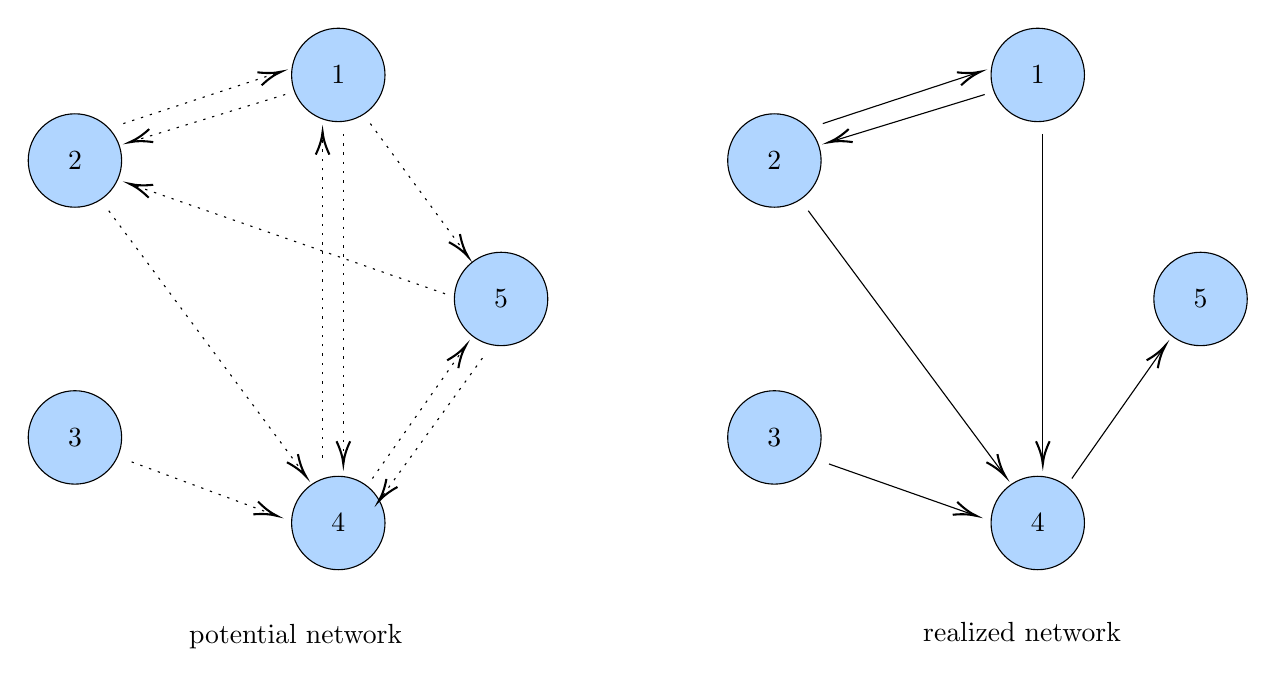
\begin{tikzpicture}[x=0.75pt,y=0.75pt,yscale=-1,xscale=1]
\draw  [fill={rgb, 255:red, 103; green, 174; blue, 255 }  ,fill opacity=0.52 ] (201.07,65.56) .. controls (201.07,53.13) and (211.15,43.06) .. (223.57,43.06) .. controls (236,43.06) and (246.07,53.13) .. (246.07,65.56) .. controls (246.07,77.98) and (236,88.06) .. (223.57,88.06) .. controls (211.15,88.06) and (201.07,77.98) .. (201.07,65.56) -- cycle ;
\draw  [fill={rgb, 255:red, 103; green, 174; blue, 255 }  ,fill opacity=0.52 ] (74.18,106.79) .. controls (74.18,94.36) and (84.25,84.29) .. (96.68,84.29) .. controls (109.1,84.29) and (119.18,94.36) .. (119.18,106.79) .. controls (119.18,119.21) and (109.1,129.29) .. (96.68,129.29) .. controls (84.25,129.29) and (74.18,119.21) .. (74.18,106.79) -- cycle ;
\draw  [fill={rgb, 255:red, 103; green, 174; blue, 255 }  ,fill opacity=0.52 ] (279.5,173.5) .. controls (279.5,161.07) and (289.57,151) .. (302,151) .. controls (314.43,151) and (324.5,161.07) .. (324.5,173.5) .. controls (324.5,185.93) and (314.43,196) .. (302,196) .. controls (289.57,196) and (279.5,185.93) .. (279.5,173.5) -- cycle ;
\draw  [fill={rgb, 255:red, 103; green, 174; blue, 255 }  ,fill opacity=0.52 ] (74.18,240.21) .. controls (74.18,227.79) and (84.25,217.71) .. (96.68,217.71) .. controls (109.1,217.71) and (119.18,227.79) .. (119.18,240.21) .. controls (119.18,252.64) and (109.1,262.71) .. (96.68,262.71) .. controls (84.25,262.71) and (74.18,252.64) .. (74.18,240.21) -- cycle ;
\draw  [fill={rgb, 255:red, 103; green, 174; blue, 255 }  ,fill opacity=0.52 ] (201.07,281.44) .. controls (201.07,269.02) and (211.15,258.94) .. (223.57,258.94) .. controls (236,258.94) and (246.07,269.02) .. (246.07,281.44) .. controls (246.07,293.87) and (236,303.94) .. (223.57,303.94) .. controls (211.15,303.94) and (201.07,293.87) .. (201.07,281.44) -- cycle ;
\draw  [dash pattern={on 0.84pt off 2.51pt}]  (239,89) -- (284.82,151.39) ;
\draw [shift={(286,153)}, rotate = 233.71] [color={rgb, 255:red, 0; green, 0; blue, 0 }  ][line width=0.75]    (10.93,-3.29) .. controls (6.95,-1.4) and (3.31,-0.3) .. (0,0) .. controls (3.31,0.3) and (6.95,1.4) .. (10.93,3.29)   ;
\draw  [dash pattern={on 0.84pt off 2.51pt}]  (198,75) -- (124.91,97.41) ;
\draw [shift={(123,98)}, rotate = 342.95] [color={rgb, 255:red, 0; green, 0; blue, 0 }  ][line width=0.75]    (10.93,-3.29) .. controls (6.95,-1.4) and (3.31,-0.3) .. (0,0) .. controls (3.31,0.3) and (6.95,1.4) .. (10.93,3.29)   ;
\draw  [dash pattern={on 0.84pt off 2.51pt}]  (226,94) -- (226,251) ;
\draw [shift={(226,253)}, rotate = 270] [color={rgb, 255:red, 0; green, 0; blue, 0 }  ][line width=0.75]    (10.93,-3.29) .. controls (6.95,-1.4) and (3.31,-0.3) .. (0,0) .. controls (3.31,0.3) and (6.95,1.4) .. (10.93,3.29)   ;
\draw  [dash pattern={on 0.84pt off 2.51pt}]  (120,89) -- (194.1,64.62) ;
\draw [shift={(196,64)}, rotate = 521.79] [color={rgb, 255:red, 0; green, 0; blue, 0 }  ][line width=0.75]    (10.93,-3.29) .. controls (6.95,-1.4) and (3.31,-0.3) .. (0,0) .. controls (3.31,0.3) and (6.95,1.4) .. (10.93,3.29)   ;
\draw  [dash pattern={on 0.84pt off 2.51pt}]  (113,131) -- (206.81,257.39) ;
\draw [shift={(208,259)}, rotate = 233.42000000000002] [color={rgb, 255:red, 0; green, 0; blue, 0 }  ][line width=0.75]    (10.93,-3.29) .. controls (6.95,-1.4) and (3.31,-0.3) .. (0,0) .. controls (3.31,0.3) and (6.95,1.4) .. (10.93,3.29)   ;
\draw  [dash pattern={on 0.84pt off 2.51pt}]  (124,252) -- (192.13,277.3) ;
\draw [shift={(194,278)}, rotate = 200.38] [color={rgb, 255:red, 0; green, 0; blue, 0 }  ][line width=0.75]    (10.93,-3.29) .. controls (6.95,-1.4) and (3.31,-0.3) .. (0,0) .. controls (3.31,0.3) and (6.95,1.4) .. (10.93,3.29)   ;
\draw  [dash pattern={on 0.84pt off 2.51pt}]  (216,250) -- (216,95) ;
\draw [shift={(216,93)}, rotate = 450] [color={rgb, 255:red, 0; green, 0; blue, 0 }  ][line width=0.75]    (10.93,-3.29) .. controls (6.95,-1.4) and (3.31,-0.3) .. (0,0) .. controls (3.31,0.3) and (6.95,1.4) .. (10.93,3.29)   ;
\draw  [dash pattern={on 0.84pt off 2.51pt}]  (240,260) -- (283.85,197.64) ;
\draw [shift={(285,196)}, rotate = 485.11] [color={rgb, 255:red, 0; green, 0; blue, 0 }  ][line width=0.75]    (10.93,-3.29) .. controls (6.95,-1.4) and (3.31,-0.3) .. (0,0) .. controls (3.31,0.3) and (6.95,1.4) .. (10.93,3.29)   ;
\draw  [dash pattern={on 0.84pt off 2.51pt}]  (293,202) -- (244.17,269.38) ;
\draw [shift={(243,271)}, rotate = 305.93] [color={rgb, 255:red, 0; green, 0; blue, 0 }  ][line width=0.75]    (10.93,-3.29) .. controls (6.95,-1.4) and (3.31,-0.3) .. (0,0) .. controls (3.31,0.3) and (6.95,1.4) .. (10.93,3.29)   ;
\draw  [dash pattern={on 0.84pt off 2.51pt}]  (275,171) -- (124.89,118.66) ;
\draw [shift={(123,118)}, rotate = 379.22] [color={rgb, 255:red, 0; green, 0; blue, 0 }  ][line width=0.75]    (10.93,-3.29) .. controls (6.95,-1.4) and (3.31,-0.3) .. (0,0) .. controls (3.31,0.3) and (6.95,1.4) .. (10.93,3.29)   ;
\draw  [fill={rgb, 255:red, 103; green, 174; blue, 255 }  ,fill opacity=0.52 ] (538.07,65.56) .. controls (538.07,53.13) and (548.15,43.06) .. (560.57,43.06) .. controls (573,43.06) and (583.07,53.13) .. (583.07,65.56) .. controls (583.07,77.98) and (573,88.06) .. (560.57,88.06) .. controls (548.15,88.06) and (538.07,77.98) .. (538.07,65.56) -- cycle ;
\draw  [fill={rgb, 255:red, 103; green, 174; blue, 255 }  ,fill opacity=0.52 ] (411.18,106.79) .. controls (411.18,94.36) and (421.25,84.29) .. (433.68,84.29) .. controls (446.1,84.29) and (456.18,94.36) .. (456.18,106.79) .. controls (456.18,119.21) and (446.1,129.29) .. (433.68,129.29) .. controls (421.25,129.29) and (411.18,119.21) .. (411.18,106.79) -- cycle ;
\draw  [fill={rgb, 255:red, 103; green, 174; blue, 255 }  ,fill opacity=0.52 ] (616.5,173.5) .. controls (616.5,161.07) and (626.57,151) .. (639,151) .. controls (651.43,151) and (661.5,161.07) .. (661.5,173.5) .. controls (661.5,185.93) and (651.43,196) .. (639,196) .. controls (626.57,196) and (616.5,185.93) .. (616.5,173.5) -- cycle ;
\draw  [fill={rgb, 255:red, 103; green, 174; blue, 255 }  ,fill opacity=0.52 ] (411.18,240.21) .. controls (411.18,227.79) and (421.25,217.71) .. (433.68,217.71) .. controls (446.1,217.71) and (456.18,227.79) .. (456.18,240.21) .. controls (456.18,252.64) and (446.1,262.71) .. (433.68,262.71) .. controls (421.25,262.71) and (411.18,252.64) .. (411.18,240.21) -- cycle ;
\draw  [fill={rgb, 255:red, 103; green, 174; blue, 255 }  ,fill opacity=0.52 ] (538.07,281.44) .. controls (538.07,269.02) and (548.15,258.94) .. (560.57,258.94) .. controls (573,258.94) and (583.07,269.02) .. (583.07,281.44) .. controls (583.07,293.87) and (573,303.94) .. (560.57,303.94) .. controls (548.15,303.94) and (538.07,293.87) .. (538.07,281.44) -- cycle ;
\draw    (535,75) -- (461.91,97.41) ;
\draw [shift={(460,98)}, rotate = 342.95] [color={rgb, 255:red, 0; green, 0; blue, 0 }  ][line width=0.75]    (10.93,-3.29) .. controls (6.95,-1.4) and (3.31,-0.3) .. (0,0) .. controls (3.31,0.3) and (6.95,1.4) .. (10.93,3.29)   ;
\draw    (563,94) -- (563,251) ;
\draw [shift={(563,253)}, rotate = 270] [color={rgb, 255:red, 0; green, 0; blue, 0 }  ][line width=0.75]    (10.93,-3.29) .. controls (6.95,-1.4) and (3.31,-0.3) .. (0,0) .. controls (3.31,0.3) and (6.95,1.4) .. (10.93,3.29)   ;
\draw    (457,89) -- (531.1,64.62) ;
\draw [shift={(533,64)}, rotate = 521.79] [color={rgb, 255:red, 0; green, 0; blue, 0 }  ][line width=0.75]    (10.93,-3.29) .. controls (6.95,-1.4) and (3.31,-0.3) .. (0,0) .. controls (3.31,0.3) and (6.95,1.4) .. (10.93,3.29)   ;
\draw    (450,131) -- (543.81,257.39) ;
\draw [shift={(545,259)}, rotate = 233.42000000000002] [color={rgb, 255:red, 0; green, 0; blue, 0 }  ][line width=0.75]    (10.93,-3.29) .. controls (6.95,-1.4) and (3.31,-0.3) .. (0,0) .. controls (3.31,0.3) and (6.95,1.4) .. (10.93,3.29)   ;
\draw    (460,253) -- (529.11,277.34) ;
\draw [shift={(531,278)}, rotate = 199.4] [color={rgb, 255:red, 0; green, 0; blue, 0 }  ][line width=0.75]    (10.93,-3.29) .. controls (6.95,-1.4) and (3.31,-0.3) .. (0,0) .. controls (3.31,0.3) and (6.95,1.4) .. (10.93,3.29)   ;
\draw    (577,260) -- (620.85,197.64) ;
\draw [shift={(622,196)}, rotate = 485.11] [color={rgb, 255:red, 0; green, 0; blue, 0 }  ][line width=0.75]    (10.93,-3.29) .. controls (6.95,-1.4) and (3.31,-0.3) .. (0,0) .. controls (3.31,0.3) and (6.95,1.4) .. (10.93,3.29)   ;
\draw (223.57,65.56) node   {$1$};
\draw (96.68,106.79) node   {$2$};
\draw (96.68,240.21) node   {$3$};
\draw (223.57,281.44) node   {$4$};
\draw (302,173.5) node   {$5$};
\draw (560.57,65.56) node   {$1$};
\draw (433.68,106.79) node   {$2$};
\draw (433.68,240.21) node   {$3$};
\draw (560.57,281.44) node   {$4$};
\draw (639,173.5) node   {$5$};
\draw (203,336) node  [align=left] {potential network};
\draw (553,334) node  [align=left] {realized network};
\end{tikzpicture}}
\caption{Difference between potential network and realized network}
\end{figure}
\end{frame}

\begin{frame}{Model : 2nd stage}
\begin{itemize}
    \item Given realized network, each agent $i = 1, \cdots, n$ simultaneously excerts an effort $x_i \ge 0$
    \item Denote $\bm{x} = (x_1, \cdots, x_n)$
    \item Payoff function is
        \[ u_i(\bm{x}, \bm{\psi}, \bm{C}, \phi) = v_i(\bm{x}, g(\bm{\psi}), \phi) - \sum_{j=1}^n g_{ij}(\bm{\psi}) c_{ij} \]
        where
        \[ v_i(\bm{x}, g(\bm{\psi}), \phi) = \alpha_i x_i - \frac{1}{2} x_i^2 + \phi \sum_{j=1}^n g_{ij}(\bm{\psi}) x_i x_j \]
    \item $\phi > 0$ and cross term represent the peer effect
    \item Optimal level of effort depends on the realized network
\end{itemize}
\end{frame}

\begin{frame}{Interpretation : Examples}
\begin{itemize}
    \item node : web sites, students
    \item link : ad on other sites, teacher-student relationship
    \item link formation cost : ad fee, psychological barrier
    \item effort : investments on web contents, effort on study
\end{itemize}
\end{frame}


\section{Equilibrium}

\begin{frame}{Equilibrium}
\begin{itemize}
    \item {\bf{Definition}} : Given $g^p$ and $\bm{C}$, the network $g^*$ is equilibrium network if $g^* = g(\bm{\psi}^*)$ where $\bm{\psi}^*$ is the strategies in the pure-strategy subgame perfect equilibrium.
    \item We focus on pure strategy equilibrium to consider the non-stochastic network
\end{itemize}
\end{frame}

\begin{frame}{2nd stage equilibrium}
\begin{itemize}
    \item {\bf{Assumption}} : $\phi \rho(\bm{G}^p) < 1$ where $\rho(\cdot)$ is spectral radius
    \item {\bf{Proposition}} : Under Assumption, for any realized network $g$, the subgame has a unique Nash equilibrium $\bm{x}^*$, which is interior and given by
    \[ \bm{x}^*(g, \phi, \bm{\alpha}) = {(\bm{I} - \phi \bm{G})}^{-1} \bm{\alpha} \]
    \item This is based on Ballester, Calv\'{o}-Armengol, and Zenou(2006)
    \item By backward induction, strategies in 1st stage also depends on $\phi$ and $\bm{\alpha}$, so we can write $\bm{\psi}(g^p, \bm{C}, \phi, \bm{\alpha})$
\end{itemize}
\end{frame}

\begin{frame}[label=theorem]{Supermodularity and equilibrium existence}
\begin{itemize}
    \item By backward induction, given 2nd stage Nash equilibrium, consider the 1st stage game as normal form game $\Gamma = \langle N, \bm{\Psi}, {(u_i)}_{i \in N} \rangle$
    \item {\bf{Theorem}} : $\Gamma$ is a supermodular game
    \begin{itemize}
        \item \hyperlink{proof}{[Proof]}
    \end{itemize}
    \item {\bf{Corollary}} : Equilibrium network always exists, in particular the greatest and smallest equilibrium network exists
    \item We focus on the greatest equilibrium network and denote $g^{**}$
    \begin{itemize}
        \item The greatest equilibrium can be obtained by well designed {\it{best response dynamics}}
    \end{itemize}
\end{itemize}
\end{frame}

\begin{frame}{Intuition}
\begin{itemize}
    \item {\bf{Strategic complementarity in 2nd stage}} : Given the realized network, if the neighbors excert more efforts, the agent has a incentive to excert more effort by peer effects.
    \item {\bf{Strategic complementarity in 1nd stage}} : When agent $i$ forms more links, he excert more effort by the strategic complementarity in 2nd stage. Agent $i$'s increased effort makes agents who have a link to him excert more effort, so all agents' level of effort weakly increases. Increasing level of efforts makes the agents to connect more agents.
\end{itemize}
\end{frame}

\begin{frame}{Toward undirected network}
\begin{itemize}
    \item {\bf{Proposition}} : If $\bm{G}^p$ and $\bm{C}$ are symmetric and $\alpha_i = \alpha > 0$ for all $i$, then $\bm{G}^*$, adjacency matrix of equilibrium network $g^*$, is symmetric
    \item We can deal with undirected network, but lack the bilateral agreement
\end{itemize}
\end{frame}

\begin{frame}{Uniqueness/Multiplicity of the equilibrium}
\begin{itemize}
    \item Equilibrium network may not be unique
    \item {\bf{Example}} : Consider $n = 2$, $\bm{\alpha} = (1, 1)$, and $\bm{G}^p = \left[
    \begin{array}{cc}
        0 & 1 \\
        1 & 0
    \end{array} \right]$.

        Then $\left[
    \begin{array}{cc}
        0 & 1 \\
        1 & 0
    \end{array} \right]$ and $\left[
    \begin{array}{cc}
        0 & 0 \\
        0 & 0
    \end{array} \right]$ can be both equilibrium network for some $c_{12}$ and $c_{21}$.
    \item Payoff matrix is:
        \begin{table}[htb]
          \begin{center}
            \begin{tabular}{|l|l|c|} \hline
              \            & $g_{21} = 1$         & $g_{21} = 0$ \\ \hline
              $g_{12} = 1$ & $\left( \frac{1}{2}{\left( \frac{1}{1 - \phi} \right)}^2 - c_{12}, \frac{1}{2}{\left( \frac{1}{1 - \phi} \right)}^2 - c_{21} \right)$ & $\left( \frac{1}{2} {(1 + \phi)}^2 - c_{12}, \frac{1}{2} \right)$ \\ \hline
              $g_{12} = 0$ & $\left( \frac{1}{2}, \frac{1}{2} {(1 + \phi)}^2 - c_{21} \right)$ & $\left( \frac{1}{2}, \frac{1}{2} \right)$ \\ \hline
            \end{tabular}
          \end{center}
        \end{table}
\end{itemize}
\end{frame}

\begin{frame}{Uniqueness/Multiplicity of the equilibrium}
\begin{figure}[h]
\centering
\tikzset{every picture/.style={line width=0.75pt}}  
\scalebox{0.6}[0.6]{     
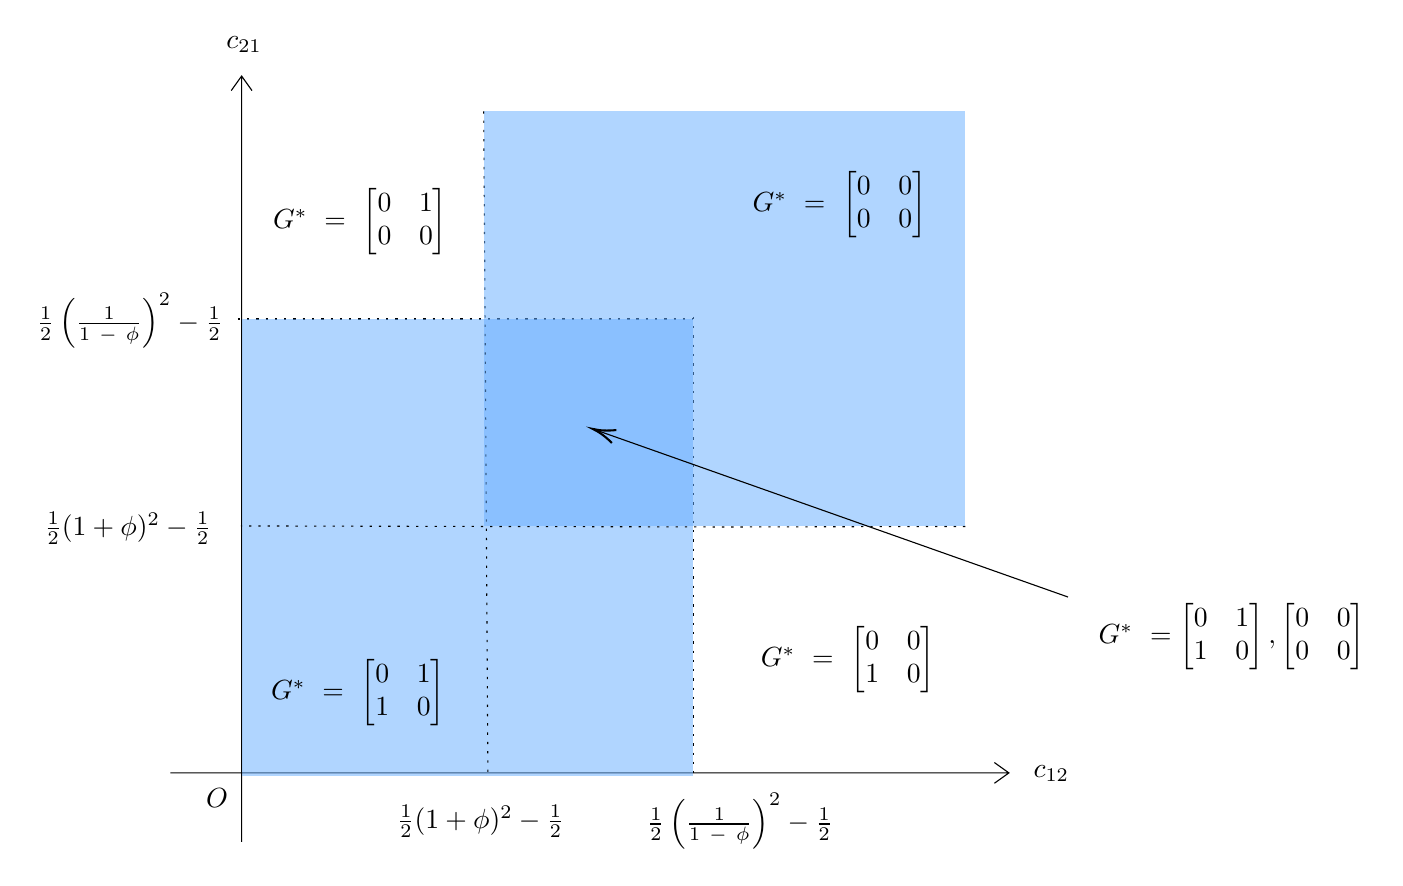
\begin{tikzpicture}[x=0.75pt,y=0.75pt,yscale=-1,xscale=1]
\draw  (115.49,390.74) -- (519.5,390.74)(149.83,55) -- (149.83,423.95) (512.5,385.74) -- (519.5,390.74) -- (512.5,395.74) (144.83,62) -- (149.83,55) -- (154.83,62)  ;
\draw [line width=0.75]  [dash pattern={on 0.84pt off 2.51pt}]  (148,172) -- (367.5,172) ;
\draw  [dash pattern={on 0.84pt off 2.51pt}]  (367.5,171) -- (367.5,392) ;
\draw  [draw opacity=0][fill={rgb, 255:red, 103; green, 174; blue, 255 }  ,fill opacity=0.52 ] (149.83,172) -- (367.5,172) -- (367.5,392) -- (149.83,392) -- cycle ;
\draw  [dash pattern={on 0.84pt off 2.51pt}]  (266.5,72) -- (268.5,392) ;
\draw  [dash pattern={on 0.84pt off 2.51pt}]  (498.5,272) -- (383.5,272.25) -- (149.5,271.75) ;
\draw  [draw opacity=0][fill={rgb, 255:red, 103; green, 174; blue, 255 }  ,fill opacity=0.52 ] (266.5,72) -- (498.5,72) -- (498.5,272) -- (266.5,272) -- cycle ;
\draw    (548,306) -- (320.89,225.67) ;
\draw [shift={(319,225)}, rotate = 379.48] [color={rgb, 255:red, 0; green, 0; blue, 0 }  ][line width=0.75]    (10.93,-3.29) .. controls (6.95,-1.4) and (3.31,-0.3) .. (0,0) .. controls (3.31,0.3) and (6.95,1.4) .. (10.93,3.29)   ;
\draw (540,391) node   {$c_{12}$};
\draw (151,40) node   {$c_{21}$};
\draw (138,403) node   {$O$};
\draw (96,173) node   {$\frac{1}{2}\left(\frac{1}{1\ -\ \phi }\right)^{2} -\frac{1}{2}$};
\draw (390,414) node   {$\frac{1}{2}\left(\frac{1}{1\ -\ \phi }\right)^{2} -\frac{1}{2}$};
\draw (95,273) node   {$\frac{1}{2}( 1+\phi )^{2} -\frac{1}{2}$};
\draw (265,414) node   {$\frac{1}{2}( 1+\phi )^{2} -\frac{1}{2}$};
\draw (438,117) node   {$G^{*} \ =\ \begin{bmatrix}
0 & 0\\
0 & 0
\end{bmatrix}$};
\draw (206,352) node   {$G^{*} \ =\ \begin{bmatrix}
0 & 1\\
1 & 0
\end{bmatrix}$};
\draw (207,125) node   {$G^{*} \ =\ \begin{bmatrix}
0 & 1\\
0 & 0
\end{bmatrix}$};
\draw (442,336) node   {$G^{*} \ =\ \begin{bmatrix}
0 & 0\\
1 & 0
\end{bmatrix}$};
\draw (627,325) node   {$G^{*} \ =\begin{bmatrix}
0 & 1\\
1 & 0
\end{bmatrix} ,\begin{bmatrix}
0 & 0\\
0 & 0
\end{bmatrix}$};
\end{tikzpicture}}
\caption{Equilibrium network region}
\end{figure}
\end{frame}

\begin{frame}{Comparative Statics}
\begin{itemize}
    \item {\bf{Proposition}} : Given the potential network $g^p$. Consider the cost $\bm{\hat{C}}$ and $\bm{C}$ with $\bm{\hat{C}} \le \bm{C}$. Then,
        \[ g^{**}(\bm{\psi}^*(g^p, \bm{\hat{C}}, \phi, \bm{\alpha})) \supseteq g^{**}(\bm{\psi}^*(g^p, \bm{C}, \phi, \bm{\alpha})) \]
    \item {\bf{Corollary}} : Given the potential network $g^p$. For $\hat{\phi} \ge \phi$ which satisfy the Assumption,
        \[ g^{**}(\bm{\psi}^*(g^p, \bm{C}, \hat{\phi}, \bm{\alpha})) \supseteq g^{**}(\bm{\psi}^*(g^p, \bm{C}, \phi, \bm{\alpha})) \]
        For $\bm{\hat{\alpha}} \ge \bm{\alpha}$,
        \[ g^{**}(\bm{\psi}^*(g^p, \bm{C}, \phi, \bm{\hat{\alpha}})) \supseteq g^{**}(\bm{\psi}^*(g^p, \bm{C}, \phi, \bm{\alpha})) \]
\end{itemize}
\end{frame}

\begin{frame}{Phase transition}
\begin{itemize}
    \item {\bf{Example}} : Suppose $n=5$, $\bm{\alpha} = (1, 1, 1, 1, 1)$, and $\phi = 1/5$
    \item $\bm{C} = \left[
            \begin{array}{ccccc}
                0 & 3 & 3 & 3 & 3 \\
                3 & 0 & 3 & 3 & 3 \\
                3 & 3 & 0 & 3 & 3 \\
                3 & 3 & 3 & 0 & 3  \\
                3 & 3 & 3 & 3 & 0
            \end{array} \right] \Rightarrow \bm{G}^{**} = \left[
            \begin{array}{ccccc}
                0 & 1 & 1 & 1 & 1 \\
                1 & 0 & 1 & 1 & 1 \\
                1 & 1 & 0 & 1 & 1 \\
                1 & 1 & 1 & 0 & 1 \\
                1 & 1 & 1 & 1 & 0
            \end{array} \right]$
    \item $\bm{\hat{C}} = \left[
            \begin{array}{ccccc}
                0 & 3 + \epsilon & 3 & 3 & 3 \\
                3 & 0 & 3 & 3 & 3 \\
                3 & 3 & 0 & 3 & 3 \\
                3 & 3 & 3 & 0 & 3  \\
                3 & 3 & 3 & 3 & 0
            \end{array} \right] \Rightarrow \bm{\hat{G}}^{**} = \left[
            \begin{array}{ccccc}
                0 & 0 & 0 & 0 & 0 \\
                0 & 0 & 0 & 0 & 0 \\
                0 & 0 & 0 & 0 & 0 \\
                0 & 0 & 0 & 0 & 0 \\
                0 & 0 & 0 & 0 & 0
            \end{array} \right]$
\end{itemize}
\end{frame}

\begin{frame}{Phase transition}
\begin{figure}[h]
\centering
\tikzset{every picture/.style={line width=0.75pt}}
\scalebox{0.7}[0.7]{     
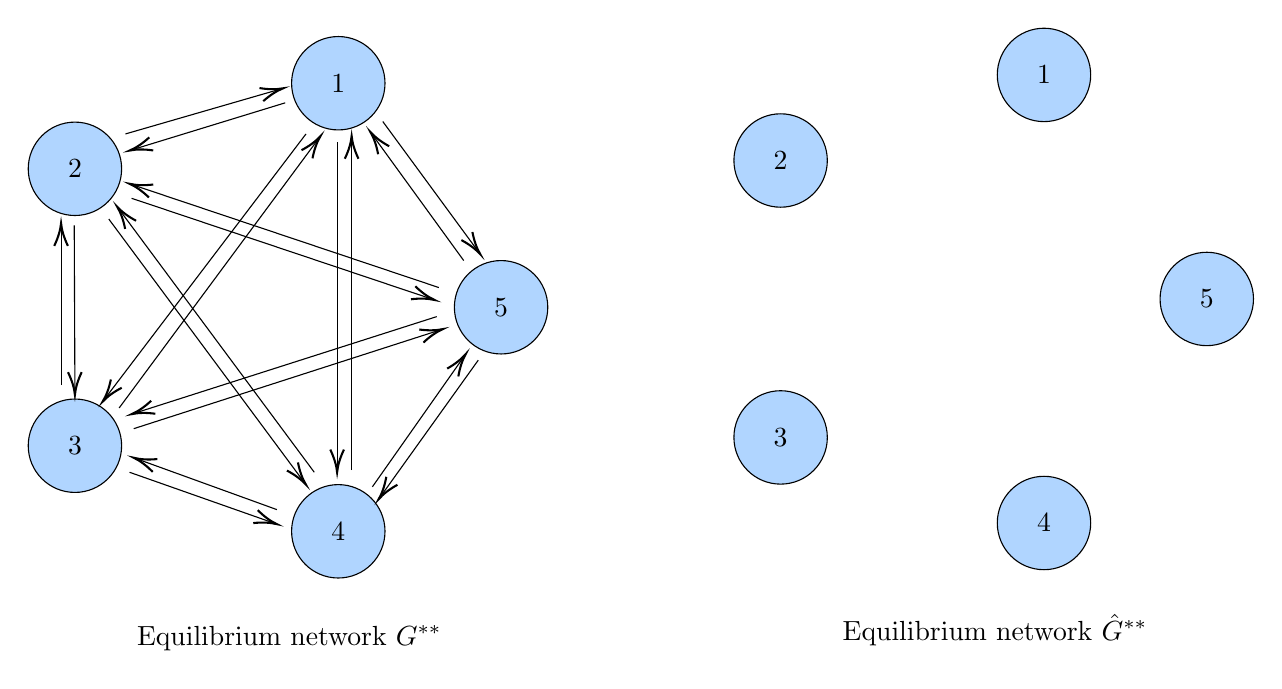
\begin{tikzpicture}[x=0.75pt,y=0.75pt,yscale=-1,xscale=1]
\draw  [fill={rgb, 255:red, 103; green, 174; blue, 255 }  ,fill opacity=0.52 ] (199.07,64.56) .. controls (199.07,52.13) and (209.15,42.06) .. (221.57,42.06) .. controls (234,42.06) and (244.07,52.13) .. (244.07,64.56) .. controls (244.07,76.98) and (234,87.06) .. (221.57,87.06) .. controls (209.15,87.06) and (199.07,76.98) .. (199.07,64.56) -- cycle ;
\draw  [fill={rgb, 255:red, 103; green, 174; blue, 255 }  ,fill opacity=0.52 ] (72.18,105.79) .. controls (72.18,93.36) and (82.25,83.29) .. (94.68,83.29) .. controls (107.1,83.29) and (117.18,93.36) .. (117.18,105.79) .. controls (117.18,118.21) and (107.1,128.29) .. (94.68,128.29) .. controls (82.25,128.29) and (72.18,118.21) .. (72.18,105.79) -- cycle ;
\draw  [fill={rgb, 255:red, 103; green, 174; blue, 255 }  ,fill opacity=0.52 ] (277.5,172.5) .. controls (277.5,160.07) and (287.57,150) .. (300,150) .. controls (312.43,150) and (322.5,160.07) .. (322.5,172.5) .. controls (322.5,184.93) and (312.43,195) .. (300,195) .. controls (287.57,195) and (277.5,184.93) .. (277.5,172.5) -- cycle ;
\draw  [fill={rgb, 255:red, 103; green, 174; blue, 255 }  ,fill opacity=0.52 ] (72.18,239.21) .. controls (72.18,226.79) and (82.25,216.71) .. (94.68,216.71) .. controls (107.1,216.71) and (117.18,226.79) .. (117.18,239.21) .. controls (117.18,251.64) and (107.1,261.71) .. (94.68,261.71) .. controls (82.25,261.71) and (72.18,251.64) .. (72.18,239.21) -- cycle ;
\draw  [fill={rgb, 255:red, 103; green, 174; blue, 255 }  ,fill opacity=0.52 ] (199.07,280.44) .. controls (199.07,268.02) and (209.15,257.94) .. (221.57,257.94) .. controls (234,257.94) and (244.07,268.02) .. (244.07,280.44) .. controls (244.07,292.87) and (234,302.94) .. (221.57,302.94) .. controls (209.15,302.94) and (199.07,292.87) .. (199.07,280.44) -- cycle ;
\draw    (196,74) -- (122.91,96.41) ;
\draw [shift={(121,97)}, rotate = 342.95] [color={rgb, 255:red, 0; green, 0; blue, 0 }  ][line width=0.75]    (10.93,-3.29) .. controls (6.95,-1.4) and (3.31,-0.3) .. (0,0) .. controls (3.31,0.3) and (6.95,1.4) .. (10.93,3.29)   ;
\draw    (221,93) -- (221,250) ;
\draw [shift={(221,252)}, rotate = 270] [color={rgb, 255:red, 0; green, 0; blue, 0 }  ][line width=0.75]    (10.93,-3.29) .. controls (6.95,-1.4) and (3.31,-0.3) .. (0,0) .. controls (3.31,0.3) and (6.95,1.4) .. (10.93,3.29)   ;
\draw    (119,89) -- (193.08,67.56) ;
\draw [shift={(195,67)}, rotate = 523.86] [color={rgb, 255:red, 0; green, 0; blue, 0 }  ][line width=0.75]    (10.93,-3.29) .. controls (6.95,-1.4) and (3.31,-0.3) .. (0,0) .. controls (3.31,0.3) and (6.95,1.4) .. (10.93,3.29)   ;
\draw    (111,130) -- (204.81,256.39) ;
\draw [shift={(206,258)}, rotate = 233.42000000000002] [color={rgb, 255:red, 0; green, 0; blue, 0 }  ][line width=0.75]    (10.93,-3.29) .. controls (6.95,-1.4) and (3.31,-0.3) .. (0,0) .. controls (3.31,0.3) and (6.95,1.4) .. (10.93,3.29)   ;
\draw    (121,252) -- (190.11,276.34) ;
\draw [shift={(192,277)}, rotate = 199.4] [color={rgb, 255:red, 0; green, 0; blue, 0 }  ][line width=0.75]    (10.93,-3.29) .. controls (6.95,-1.4) and (3.31,-0.3) .. (0,0) .. controls (3.31,0.3) and (6.95,1.4) .. (10.93,3.29)   ;
\draw    (238,259) -- (281.85,196.64) ;
\draw [shift={(283,195)}, rotate = 485.11] [color={rgb, 255:red, 0; green, 0; blue, 0 }  ][line width=0.75]    (10.93,-3.29) .. controls (6.95,-1.4) and (3.31,-0.3) .. (0,0) .. controls (3.31,0.3) and (6.95,1.4) .. (10.93,3.29)   ;
\draw    (243,83) -- (288.82,145.39) ;
\draw [shift={(290,147)}, rotate = 233.71] [color={rgb, 255:red, 0; green, 0; blue, 0 }  ][line width=0.75]    (10.93,-3.29) .. controls (6.95,-1.4) and (3.31,-0.3) .. (0,0) .. controls (3.31,0.3) and (6.95,1.4) .. (10.93,3.29)   ;
\draw    (206,89) -- (109.21,216.41) ;
\draw [shift={(108,218)}, rotate = 307.22] [color={rgb, 255:red, 0; green, 0; blue, 0 }  ][line width=0.75]    (10.93,-3.29) .. controls (6.95,-1.4) and (3.31,-0.3) .. (0,0) .. controls (3.31,0.3) and (6.95,1.4) .. (10.93,3.29)   ;
\draw    (94.35,133) -- (94.67,212.71) ;
\draw [shift={(94.68,214.71)}, rotate = 269.77] [color={rgb, 255:red, 0; green, 0; blue, 0 }  ][line width=0.75]    (10.93,-3.29) .. controls (6.95,-1.4) and (3.31,-0.3) .. (0,0) .. controls (3.31,0.3) and (6.95,1.4) .. (10.93,3.29)   ;
\draw    (122,120) -- (266.1,168.36) ;
\draw [shift={(268,169)}, rotate = 198.55] [color={rgb, 255:red, 0; green, 0; blue, 0 }  ][line width=0.75]    (10.93,-3.29) .. controls (6.95,-1.4) and (3.31,-0.3) .. (0,0) .. controls (3.31,0.3) and (6.95,1.4) .. (10.93,3.29)   ;
\draw    (116,221) -- (211.81,91.61) ;
\draw [shift={(213,90)}, rotate = 486.52] [color={rgb, 255:red, 0; green, 0; blue, 0 }  ][line width=0.75]    (10.93,-3.29) .. controls (6.95,-1.4) and (3.31,-0.3) .. (0,0) .. controls (3.31,0.3) and (6.95,1.4) .. (10.93,3.29)   ;
\draw    (88,210) -- (88,134) ;
\draw [shift={(88,132)}, rotate = 450] [color={rgb, 255:red, 0; green, 0; blue, 0 }  ][line width=0.75]    (10.93,-3.29) .. controls (6.95,-1.4) and (3.31,-0.3) .. (0,0) .. controls (3.31,0.3) and (6.95,1.4) .. (10.93,3.29)   ;
\draw    (123,231) -- (270.1,183.61) ;
\draw [shift={(272,183)}, rotate = 522.14] [color={rgb, 255:red, 0; green, 0; blue, 0 }  ][line width=0.75]    (10.93,-3.29) .. controls (6.95,-1.4) and (3.31,-0.3) .. (0,0) .. controls (3.31,0.3) and (6.95,1.4) .. (10.93,3.29)   ;
\draw    (228,251) -- (228,92) ;
\draw [shift={(228,90)}, rotate = 450] [color={rgb, 255:red, 0; green, 0; blue, 0 }  ][line width=0.75]    (10.93,-3.29) .. controls (6.95,-1.4) and (3.31,-0.3) .. (0,0) .. controls (3.31,0.3) and (6.95,1.4) .. (10.93,3.29)   ;
\draw    (116.19,125.61) -- (210,252) ;
\draw [shift={(115,124)}, rotate = 53.42] [color={rgb, 255:red, 0; green, 0; blue, 0 }  ][line width=0.75]    (10.93,-3.29) .. controls (6.95,-1.4) and (3.31,-0.3) .. (0,0) .. controls (3.31,0.3) and (6.95,1.4) .. (10.93,3.29)   ;
\draw    (192,270) -- (124.88,245.68) ;
\draw [shift={(123,245)}, rotate = 379.91999999999996] [color={rgb, 255:red, 0; green, 0; blue, 0 }  ][line width=0.75]    (10.93,-3.29) .. controls (6.95,-1.4) and (3.31,-0.3) .. (0,0) .. controls (3.31,0.3) and (6.95,1.4) .. (10.93,3.29)   ;
\draw    (282,150) -- (238.17,89.62) ;
\draw [shift={(237,88)}, rotate = 414.03] [color={rgb, 255:red, 0; green, 0; blue, 0 }  ][line width=0.75]    (10.93,-3.29) .. controls (6.95,-1.4) and (3.31,-0.3) .. (0,0) .. controls (3.31,0.3) and (6.95,1.4) .. (10.93,3.29)   ;
\draw    (270,163) -- (122.9,113.64) ;
\draw [shift={(121,113)}, rotate = 378.55] [color={rgb, 255:red, 0; green, 0; blue, 0 }  ][line width=0.75]    (10.93,-3.29) .. controls (6.95,-1.4) and (3.31,-0.3) .. (0,0) .. controls (3.31,0.3) and (6.95,1.4) .. (10.93,3.29)   ;
\draw    (269,177) -- (123.9,223.39) ;
\draw [shift={(122,224)}, rotate = 342.27] [color={rgb, 255:red, 0; green, 0; blue, 0 }  ][line width=0.75]    (10.93,-3.29) .. controls (6.95,-1.4) and (3.31,-0.3) .. (0,0) .. controls (3.31,0.3) and (6.95,1.4) .. (10.93,3.29)   ;
\draw    (289,198) -- (242.16,263.37) ;
\draw [shift={(241,265)}, rotate = 305.62] [color={rgb, 255:red, 0; green, 0; blue, 0 }  ][line width=0.75]    (10.93,-3.29) .. controls (6.95,-1.4) and (3.31,-0.3) .. (0,0) .. controls (3.31,0.3) and (6.95,1.4) .. (10.93,3.29)   ;
\draw  [fill={rgb, 255:red, 103; green, 174; blue, 255 }  ,fill opacity=0.52 ] (539.07,60.56) .. controls (539.07,48.13) and (549.15,38.06) .. (561.57,38.06) .. controls (574,38.06) and (584.07,48.13) .. (584.07,60.56) .. controls (584.07,72.98) and (574,83.06) .. (561.57,83.06) .. controls (549.15,83.06) and (539.07,72.98) .. (539.07,60.56) -- cycle ;
\draw  [fill={rgb, 255:red, 103; green, 174; blue, 255 }  ,fill opacity=0.52 ] (412.18,101.79) .. controls (412.18,89.36) and (422.25,79.29) .. (434.68,79.29) .. controls (447.1,79.29) and (457.18,89.36) .. (457.18,101.79) .. controls (457.18,114.21) and (447.1,124.29) .. (434.68,124.29) .. controls (422.25,124.29) and (412.18,114.21) .. (412.18,101.79) -- cycle ;
\draw  [fill={rgb, 255:red, 103; green, 174; blue, 255 }  ,fill opacity=0.52 ] (617.5,168.5) .. controls (617.5,156.07) and (627.57,146) .. (640,146) .. controls (652.43,146) and (662.5,156.07) .. (662.5,168.5) .. controls (662.5,180.93) and (652.43,191) .. (640,191) .. controls (627.57,191) and (617.5,180.93) .. (617.5,168.5) -- cycle ;
\draw  [fill={rgb, 255:red, 103; green, 174; blue, 255 }  ,fill opacity=0.52 ] (412.18,235.21) .. controls (412.18,222.79) and (422.25,212.71) .. (434.68,212.71) .. controls (447.1,212.71) and (457.18,222.79) .. (457.18,235.21) .. controls (457.18,247.64) and (447.1,257.71) .. (434.68,257.71) .. controls (422.25,257.71) and (412.18,247.64) .. (412.18,235.21) -- cycle ;
\draw  [fill={rgb, 255:red, 103; green, 174; blue, 255 }  ,fill opacity=0.52 ] (539.07,276.44) .. controls (539.07,264.02) and (549.15,253.94) .. (561.57,253.94) .. controls (574,253.94) and (584.07,264.02) .. (584.07,276.44) .. controls (584.07,288.87) and (574,298.94) .. (561.57,298.94) .. controls (549.15,298.94) and (539.07,288.87) .. (539.07,276.44) -- cycle ;
\draw (221.57,64.56) node   {$1$};
\draw (94.68,105.79) node   {$2$};
\draw (94.68,239.21) node   {$3$};
\draw (221.57,280.44) node   {$4$};
\draw (300,172.5) node   {$5$};
\draw (198,332) node  [align=left] {Equilibrium network $\displaystyle G^{**}$};
\draw (561.57,60.56) node   {$1$};
\draw (434.68,101.79) node   {$2$};
\draw (434.68,235.21) node   {$3$};
\draw (561.57,276.44) node   {$4$};
\draw (640,168.5) node   {$5$};
\draw (538,328) node  [align=left] {Equilibrium network $\displaystyle \hat{G}^{**}$};
\end{tikzpicture}}
\caption{Equilibrium networks}
\end{figure}
\end{frame}


\section{Policy Implication}

\begin{frame}{Key player}
\begin{itemize}
    \item Key player is the agent who has the largest impact on the aggregate behavior of the network
    \item {\bf{Definition}} : Agent $i$ is key player in exogenous network $g$ if, given network $g$,
        \[ i \in \arg \max_{i \in N} \{ x^*(g) - x^*(g^{-i}) \} \]
        where $x^*(g) = \sum_{i=1}^n x_i^*(g)$ and $g^{-i}$ is the network where agent $i$ is removed from the network $g$
\end{itemize}
\end{frame}

\begin{frame}{Key player in endogenous network}
\begin{itemize}
    \item {\bf{Definition}} : Agent $i$ is key player in endogenous network if, given potential network $g^p$,
        \[ i \in \arg \max_{i \in N} \{ x^*(g^{**}(\bm{\psi}({g^p}, \bm{C}))) - x^*(g^{**}(\bm{\psi}({g^p}^{-i}, \bm{C}^{-i}))) \} \]
        where ${g^p}^{-i}$ is the network where agent $i$ is removed from the network $g^p$
    \item However, it is difficult to identify key player due to the complexity of the mapping from cost structure to realized network
\end{itemize}
\end{frame}

\begin{frame}{Difference bet. endogenous and exogenous key player}
\begin{itemize}
    \item {\bf{Example}} : Suppose $n=5$, $\bm{\alpha} = (1, 1, 1, 1, 1)$ and $\phi = 1/5$
    \item $\bm{C} = \left[
            \begin{array}{ccccc}
                0 & 3.6 & 0.2 & 0.2 & 0.2 \\
                0.3 & 0 & 0.2 & 0.5 & 5.5 \\
                0.2 & 0.2 & 0 & 4.5 & 4.3 \\
                4.1 & 0.2 & 0.4 & 0 & 6.5 \\
                3.2 & 4.1 & 0.3 & 1.0 & 0
            \end{array} \right] \Rightarrow \bm{G}^{**} = \left[
            \begin{array}{ccccc}
                0 & 0 & 1 & 1 & 1 \\
                1 & 0 & 1 & 1 & 0 \\
                1 & 1 & 0 & 0 & 0 \\
                0 & 1 & 1 & 0 & 0 \\
                0 & 0 & 1 & 0 & 0
            \end{array} \right]$
    \item Then,
        \begin{table}[htb]
          \begin{center}
            \begin{tabular}{|l|l|c|} \hline
              agent $1$ & $x_1^* = 1.99541284$ & key player in endogenous network \\ \hline
              agent $2$ & $x_2^* = 2.12155963$ & agent with highest effort \\ \hline
              agent $3$ & $x_3^* = 1.82339450$  & key player in exogenous network \\ \hline
              agent $4$ & $x_4^* = 1.78899083$ & \  \\ \hline
              agent $5$ & $x_5^* = 1.36467890$ & \ \\ \hline
            \end{tabular}
          \end{center}
        \end{table}
\end{itemize}
\end{frame}

\begin{frame}{Diff bet. endogenous and exogenous key player}
\begin{figure}[h]
\raggedleft
\tikzset{every picture/.style={line width=0.75pt}}
\scalebox{0.75}[0.75]{   
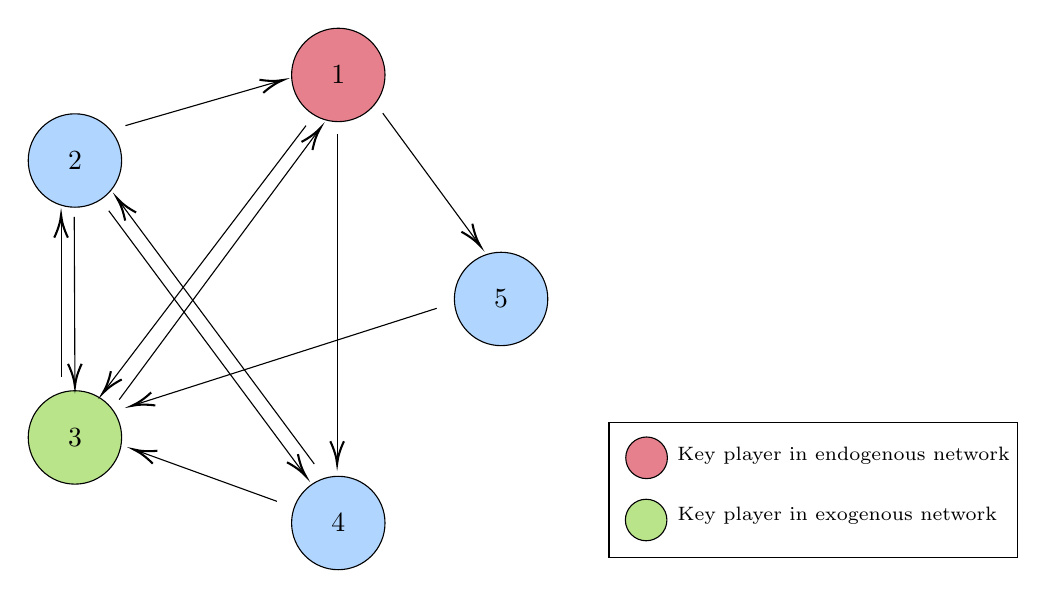
\begin{tikzpicture}[x=0.75pt,y=0.75pt,yscale=-1,xscale=1]
\draw  [fill={rgb, 255:red, 208; green, 2; blue, 27 }  ,fill opacity=0.5 ] (416.07,67.56) .. controls (416.07,55.13) and (426.15,45.06) .. (438.57,45.06) .. controls (451,45.06) and (461.07,55.13) .. (461.07,67.56) .. controls (461.07,79.98) and (451,90.06) .. (438.57,90.06) .. controls (426.15,90.06) and (416.07,79.98) .. (416.07,67.56) -- cycle ;
\draw  [fill={rgb, 255:red, 103; green, 174; blue, 255 }  ,fill opacity=0.52 ] (289.18,108.79) .. controls (289.18,96.36) and (299.25,86.29) .. (311.68,86.29) .. controls (324.1,86.29) and (334.18,96.36) .. (334.18,108.79) .. controls (334.18,121.21) and (324.1,131.29) .. (311.68,131.29) .. controls (299.25,131.29) and (289.18,121.21) .. (289.18,108.79) -- cycle ;
\draw  [fill={rgb, 255:red, 103; green, 174; blue, 255 }  ,fill opacity=0.52 ] (494.5,175.5) .. controls (494.5,163.07) and (504.57,153) .. (517,153) .. controls (529.43,153) and (539.5,163.07) .. (539.5,175.5) .. controls (539.5,187.93) and (529.43,198) .. (517,198) .. controls (504.57,198) and (494.5,187.93) .. (494.5,175.5) -- cycle ;
\draw  [fill={rgb, 255:red, 115; green, 201; blue, 21 }  ,fill opacity=0.5 ] (289.18,242.21) .. controls (289.18,229.79) and (299.25,219.71) .. (311.68,219.71) .. controls (324.1,219.71) and (334.18,229.79) .. (334.18,242.21) .. controls (334.18,254.64) and (324.1,264.71) .. (311.68,264.71) .. controls (299.25,264.71) and (289.18,254.64) .. (289.18,242.21) -- cycle ;
\draw  [fill={rgb, 255:red, 103; green, 174; blue, 255 }  ,fill opacity=0.52 ] (416.07,283.44) .. controls (416.07,271.02) and (426.15,260.94) .. (438.57,260.94) .. controls (451,260.94) and (461.07,271.02) .. (461.07,283.44) .. controls (461.07,295.87) and (451,305.94) .. (438.57,305.94) .. controls (426.15,305.94) and (416.07,295.87) .. (416.07,283.44) -- cycle ;
\draw    (438,96) -- (438,253) ;
\draw [shift={(438,255)}, rotate = 270] [color={rgb, 255:red, 0; green, 0; blue, 0 }  ][line width=0.75]    (10.93,-3.29) .. controls (6.95,-1.4) and (3.31,-0.3) .. (0,0) .. controls (3.31,0.3) and (6.95,1.4) .. (10.93,3.29)   ;
\draw    (336,92) -- (410.08,70.56) ;
\draw [shift={(412,70)}, rotate = 523.86] [color={rgb, 255:red, 0; green, 0; blue, 0 }  ][line width=0.75]    (10.93,-3.29) .. controls (6.95,-1.4) and (3.31,-0.3) .. (0,0) .. controls (3.31,0.3) and (6.95,1.4) .. (10.93,3.29)   ;
\draw    (328,133) -- (421.81,259.39) ;
\draw [shift={(423,261)}, rotate = 233.42000000000002] [color={rgb, 255:red, 0; green, 0; blue, 0 }  ][line width=0.75]    (10.93,-3.29) .. controls (6.95,-1.4) and (3.31,-0.3) .. (0,0) .. controls (3.31,0.3) and (6.95,1.4) .. (10.93,3.29)   ;
\draw    (460,86) -- (505.82,148.39) ;
\draw [shift={(507,150)}, rotate = 233.71] [color={rgb, 255:red, 0; green, 0; blue, 0 }  ][line width=0.75]    (10.93,-3.29) .. controls (6.95,-1.4) and (3.31,-0.3) .. (0,0) .. controls (3.31,0.3) and (6.95,1.4) .. (10.93,3.29)   ;
\draw    (423,92) -- (326.21,219.41) ;
\draw [shift={(325,221)}, rotate = 307.22] [color={rgb, 255:red, 0; green, 0; blue, 0 }  ][line width=0.75]    (10.93,-3.29) .. controls (6.95,-1.4) and (3.31,-0.3) .. (0,0) .. controls (3.31,0.3) and (6.95,1.4) .. (10.93,3.29)   ;
\draw    (311.35,136) -- (311.67,215.71) ;
\draw [shift={(311.68,217.71)}, rotate = 269.77] [color={rgb, 255:red, 0; green, 0; blue, 0 }  ][line width=0.75]    (10.93,-3.29) .. controls (6.95,-1.4) and (3.31,-0.3) .. (0,0) .. controls (3.31,0.3) and (6.95,1.4) .. (10.93,3.29)   ;
\draw    (333,224) -- (428.81,94.61) ;
\draw [shift={(430,93)}, rotate = 486.52] [color={rgb, 255:red, 0; green, 0; blue, 0 }  ][line width=0.75]    (10.93,-3.29) .. controls (6.95,-1.4) and (3.31,-0.3) .. (0,0) .. controls (3.31,0.3) and (6.95,1.4) .. (10.93,3.29)   ;
\draw    (305,213) -- (305,137) ;
\draw [shift={(305,135)}, rotate = 450] [color={rgb, 255:red, 0; green, 0; blue, 0 }  ][line width=0.75]    (10.93,-3.29) .. controls (6.95,-1.4) and (3.31,-0.3) .. (0,0) .. controls (3.31,0.3) and (6.95,1.4) .. (10.93,3.29)   ;
\draw    (333.19,128.61) -- (427,255) ;
\draw [shift={(332,127)}, rotate = 53.42] [color={rgb, 255:red, 0; green, 0; blue, 0 }  ][line width=0.75]    (10.93,-3.29) .. controls (6.95,-1.4) and (3.31,-0.3) .. (0,0) .. controls (3.31,0.3) and (6.95,1.4) .. (10.93,3.29)   ;
\draw    (409,273) -- (341.88,248.68) ;
\draw [shift={(340,248)}, rotate = 379.91999999999996] [color={rgb, 255:red, 0; green, 0; blue, 0 }  ][line width=0.75]    (10.93,-3.29) .. controls (6.95,-1.4) and (3.31,-0.3) .. (0,0) .. controls (3.31,0.3) and (6.95,1.4) .. (10.93,3.29)   ;
\draw    (486,180) -- (340.9,226.39) ;
\draw [shift={(339,227)}, rotate = 342.27] [color={rgb, 255:red, 0; green, 0; blue, 0 }  ][line width=0.75]    (10.93,-3.29) .. controls (6.95,-1.4) and (3.31,-0.3) .. (0,0) .. controls (3.31,0.3) and (6.95,1.4) .. (10.93,3.29)   ;
\draw   (569,235) -- (766,235) -- (766,300) -- (569,300) -- cycle ;
\draw  [fill={rgb, 255:red, 208; green, 2; blue, 27 }  ,fill opacity=0.5 ] (577.07,252.03) .. controls (577.07,246.49) and (581.56,242) .. (587.1,242) .. controls (592.64,242) and (597.13,246.49) .. (597.13,252.03) .. controls (597.13,257.57) and (592.64,262.06) .. (587.1,262.06) .. controls (581.56,262.06) and (577.07,257.57) .. (577.07,252.03) -- cycle ;
\draw  [fill={rgb, 255:red, 115; green, 201; blue, 21 }  ,fill opacity=0.5 ] (576.89,282) .. controls (576.89,276.48) and (581.37,272) .. (586.89,272) .. controls (592.41,272) and (596.89,276.48) .. (596.89,282) .. controls (596.89,287.52) and (592.41,292) .. (586.89,292) .. controls (581.37,292) and (576.89,287.52) .. (576.89,282) -- cycle ;
\draw (438.57,67.56) node   {$1$};
\draw (311.68,108.79) node   {$2$};
\draw (311.68,242.21) node   {$3$};
\draw (438.57,283.44) node   {$4$};
\draw (517,175.5) node   {$5$};
\draw (682,251) node  [align=left] {{\scriptsize Key player in endogenous network}};
\draw (679,280) node  [align=left] {{\scriptsize Key player in exogenous network}};
\end{tikzpicture}}
\caption{Equilibrium network $G^{**}$ and key players}
\end{figure}
\end{frame}

\begin{frame}{Key removing link in endogenous and exogenous network}
\begin{itemize}
    \item {\bf{Definition}} : Link $ij$ is key removing link in endogenous network if, given potential network $g^p$,
        \[ ij \in \arg \max_{ij \in E(g^p)} \{ x^*(g^{**}(\bm{\psi}(g^p, \bm{C}))) - x^*(g^{**}(\bm{\psi}({g^p}^{-ij}, \bm{C}))) \} \]
        where $E(g)$ is the set of links in $g^p$ and ${g^p}^{-ij}$ is network obtained by removing link $ij$ from $g^p$
    \item {\bf{Definition}} : Link $ij$ is key removing link in exogenous network $g$ if, given network $g$,
        \[ ij \in \arg \max_{ij \in E(g)} \{ x^*(g) - x^*(g^{-ij}) \} \]
        where $E(g)$ is the set of links in $g$ and $g^{-ij}$ is network obtained by removing link $ij$ from $g$
\end{itemize}
\end{frame}

\begin{frame}{Diff bet. endogenous and exogenous key removing link}
\begin{itemize}
    \item {\bf{Example}} : Suppose $n=3$, $\bm{\alpha} = (1,1,1)$ and $\phi = 1/3$
    \item Potential network is $\bm{G}^p = \left[
                                    \begin{array}{ccc}
                                        0 & 1 & 1 \\
                                        1 & 0 & 1 \\
                                        1 & 0 & 0
                                    \end{array} \right]$
    \item $\bm{C} = \left[
                \begin{array}{ccc}
                    0 & 1 & 1 \\
                    1 & 0 & 1 \\
                    1 & 0 & 0
                \end{array} \right] \Rightarrow
            \bm{G}^{**} = \left[
                \begin{array}{ccc}
                    0 & 1 & 1 \\
                    1 & 0 & 1 \\
                    1 & 0 & 0
                \end{array} \right]$
    \item Then,
        \begin{itemize}
            \item Key removing link in endogenous network is $\bm{23}$
            \item Key removing link in exogenous network is $\bm{12}$ and $\bm{31}$
        \end{itemize}
\end{itemize}
\end{frame}

\begin{frame}{Diff bet. endogenous and exogenous key removing link}
\begin{figure}[h]
\centering
\tikzset{every picture/.style={line width=0.75pt}}       
\scalebox{0.5}[0.5]{
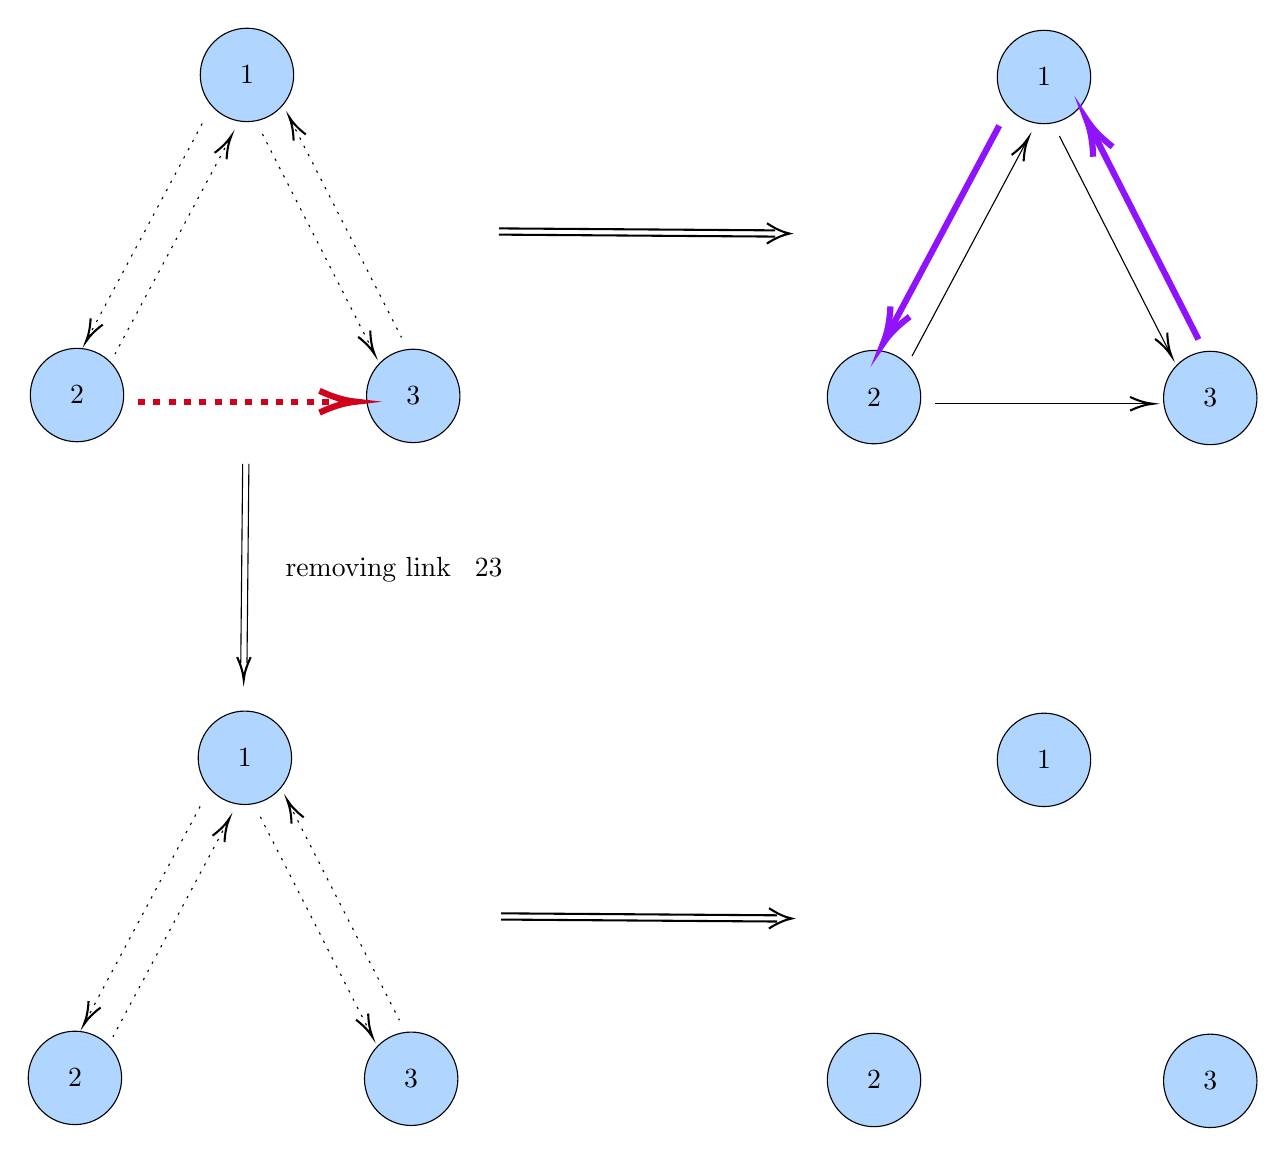
\begin{tikzpicture}[x=0.75pt,y=0.75pt,yscale=-1,xscale=1]
\draw  [fill={rgb, 255:red, 103; green, 174; blue, 255 }  ,fill opacity=0.52 ] (170.07,34.56) .. controls (170.07,22.13) and (180.15,12.06) .. (192.57,12.06) .. controls (205,12.06) and (215.07,22.13) .. (215.07,34.56) .. controls (215.07,46.98) and (205,57.06) .. (192.57,57.06) .. controls (180.15,57.06) and (170.07,46.98) .. (170.07,34.56) -- cycle ;
\draw  [fill={rgb, 255:red, 103; green, 174; blue, 255 }  ,fill opacity=0.52 ] (88.18,188.79) .. controls (88.18,176.36) and (98.25,166.29) .. (110.68,166.29) .. controls (123.1,166.29) and (133.18,176.36) .. (133.18,188.79) .. controls (133.18,201.21) and (123.1,211.29) .. (110.68,211.29) .. controls (98.25,211.29) and (88.18,201.21) .. (88.18,188.79) -- cycle ;
\draw  [fill={rgb, 255:red, 103; green, 174; blue, 255 }  ,fill opacity=0.52 ] (250.18,189.21) .. controls (250.18,176.79) and (260.25,166.71) .. (272.68,166.71) .. controls (285.1,166.71) and (295.18,176.79) .. (295.18,189.21) .. controls (295.18,201.64) and (285.1,211.71) .. (272.68,211.71) .. controls (260.25,211.71) and (250.18,201.64) .. (250.18,189.21) -- cycle ;
\draw  [dash pattern={on 0.84pt off 2.51pt}]  (171,58) -- (115.94,161.24) ;
\draw [shift={(115,163)}, rotate = 298.07] [color={rgb, 255:red, 0; green, 0; blue, 0 }  ][line width=0.75]    (10.93,-3.29) .. controls (6.95,-1.4) and (3.31,-0.3) .. (0,0) .. controls (3.31,0.3) and (6.95,1.4) .. (10.93,3.29)   ;
\draw  [dash pattern={on 0.84pt off 2.51pt}]  (184.06,65.76) -- (129,169) ;
\draw [shift={(185,64)}, rotate = 118.07] [color={rgb, 255:red, 0; green, 0; blue, 0 }  ][line width=0.75]    (10.93,-3.29) .. controls (6.95,-1.4) and (3.31,-0.3) .. (0,0) .. controls (3.31,0.3) and (6.95,1.4) .. (10.93,3.29)   ;
\draw  [dash pattern={on 0.84pt off 2.51pt}]  (200,63) -- (253.09,167.22) ;
\draw [shift={(254,169)}, rotate = 243] [color={rgb, 255:red, 0; green, 0; blue, 0 }  ][line width=0.75]    (10.93,-3.29) .. controls (6.95,-1.4) and (3.31,-0.3) .. (0,0) .. controls (3.31,0.3) and (6.95,1.4) .. (10.93,3.29)   ;
\draw  [dash pattern={on 0.84pt off 2.51pt}]  (213.91,56.78) -- (267,161) ;
\draw [shift={(213,55)}, rotate = 63] [color={rgb, 255:red, 0; green, 0; blue, 0 }  ][line width=0.75]    (10.93,-3.29) .. controls (6.95,-1.4) and (3.31,-0.3) .. (0,0) .. controls (3.31,0.3) and (6.95,1.4) .. (10.93,3.29)   ;
\draw [color={rgb, 255:red, 208; green, 2; blue, 27 }  ,draw opacity=1 ][line width=2.25]  [dash pattern={on 2.53pt off 3.02pt}]  (140,192) -- (241,192) ;
\draw [shift={(245,192)}, rotate = 180] [color={rgb, 255:red, 208; green, 2; blue, 27 }  ,draw opacity=1 ][line width=2.25]    (17.49,-5.26) .. controls (11.12,-2.23) and (5.29,-0.48) .. (0,0) .. controls (5.29,0.48) and (11.12,2.23) .. (17.49,5.26)   ;
\draw  [fill={rgb, 255:red, 103; green, 174; blue, 255 }  ,fill opacity=0.52 ] (169.07,363.56) .. controls (169.07,351.13) and (179.15,341.06) .. (191.57,341.06) .. controls (204,341.06) and (214.07,351.13) .. (214.07,363.56) .. controls (214.07,375.98) and (204,386.06) .. (191.57,386.06) .. controls (179.15,386.06) and (169.07,375.98) .. (169.07,363.56) -- cycle ;
\draw  [fill={rgb, 255:red, 103; green, 174; blue, 255 }  ,fill opacity=0.52 ] (87.18,517.79) .. controls (87.18,505.36) and (97.25,495.29) .. (109.68,495.29) .. controls (122.1,495.29) and (132.18,505.36) .. (132.18,517.79) .. controls (132.18,530.21) and (122.1,540.29) .. (109.68,540.29) .. controls (97.25,540.29) and (87.18,530.21) .. (87.18,517.79) -- cycle ;
\draw  [fill={rgb, 255:red, 103; green, 174; blue, 255 }  ,fill opacity=0.52 ] (249.18,518.21) .. controls (249.18,505.79) and (259.25,495.71) .. (271.68,495.71) .. controls (284.1,495.71) and (294.18,505.79) .. (294.18,518.21) .. controls (294.18,530.64) and (284.1,540.71) .. (271.68,540.71) .. controls (259.25,540.71) and (249.18,530.64) .. (249.18,518.21) -- cycle ;
\draw  [dash pattern={on 0.84pt off 2.51pt}]  (170,387) -- (114.94,490.24) ;
\draw [shift={(114,492)}, rotate = 298.07] [color={rgb, 255:red, 0; green, 0; blue, 0 }  ][line width=0.75]    (10.93,-3.29) .. controls (6.95,-1.4) and (3.31,-0.3) .. (0,0) .. controls (3.31,0.3) and (6.95,1.4) .. (10.93,3.29)   ;
\draw  [dash pattern={on 0.84pt off 2.51pt}]  (183.06,394.76) -- (128,498) ;
\draw [shift={(184,393)}, rotate = 118.07] [color={rgb, 255:red, 0; green, 0; blue, 0 }  ][line width=0.75]    (10.93,-3.29) .. controls (6.95,-1.4) and (3.31,-0.3) .. (0,0) .. controls (3.31,0.3) and (6.95,1.4) .. (10.93,3.29)   ;
\draw  [dash pattern={on 0.84pt off 2.51pt}]  (199,392) -- (252.09,496.22) ;
\draw [shift={(253,498)}, rotate = 243] [color={rgb, 255:red, 0; green, 0; blue, 0 }  ][line width=0.75]    (10.93,-3.29) .. controls (6.95,-1.4) and (3.31,-0.3) .. (0,0) .. controls (3.31,0.3) and (6.95,1.4) .. (10.93,3.29)   ;
\draw  [dash pattern={on 0.84pt off 2.51pt}]  (212.91,385.78) -- (266,490) ;
\draw [shift={(212,384)}, rotate = 63] [color={rgb, 255:red, 0; green, 0; blue, 0 }  ][line width=0.75]    (10.93,-3.29) .. controls (6.95,-1.4) and (3.31,-0.3) .. (0,0) .. controls (3.31,0.3) and (6.95,1.4) .. (10.93,3.29)   ;
\draw  [fill={rgb, 255:red, 103; green, 174; blue, 255 }  ,fill opacity=0.52 ] (554.07,35.56) .. controls (554.07,23.13) and (564.15,13.06) .. (576.57,13.06) .. controls (589,13.06) and (599.07,23.13) .. (599.07,35.56) .. controls (599.07,47.98) and (589,58.06) .. (576.57,58.06) .. controls (564.15,58.06) and (554.07,47.98) .. (554.07,35.56) -- cycle ;
\draw  [fill={rgb, 255:red, 103; green, 174; blue, 255 }  ,fill opacity=0.52 ] (472.18,189.79) .. controls (472.18,177.36) and (482.25,167.29) .. (494.68,167.29) .. controls (507.1,167.29) and (517.18,177.36) .. (517.18,189.79) .. controls (517.18,202.21) and (507.1,212.29) .. (494.68,212.29) .. controls (482.25,212.29) and (472.18,202.21) .. (472.18,189.79) -- cycle ;
\draw  [fill={rgb, 255:red, 103; green, 174; blue, 255 }  ,fill opacity=0.52 ] (634.18,190.21) .. controls (634.18,177.79) and (644.25,167.71) .. (656.68,167.71) .. controls (669.1,167.71) and (679.18,177.79) .. (679.18,190.21) .. controls (679.18,202.64) and (669.1,212.71) .. (656.68,212.71) .. controls (644.25,212.71) and (634.18,202.64) .. (634.18,190.21) -- cycle ;
\draw [color={rgb, 255:red, 144; green, 19; blue, 254 }  ,draw opacity=1 ][line width=2.25]    (555,59) -- (500.88,160.47) ;
\draw [shift={(499,164)}, rotate = 298.07] [color={rgb, 255:red, 144; green, 19; blue, 254 }  ,draw opacity=1 ][line width=2.25]    (17.49,-5.26) .. controls (11.12,-2.23) and (5.29,-0.48) .. (0,0) .. controls (5.29,0.48) and (11.12,2.23) .. (17.49,5.26)   ;
\draw    (568.06,66.76) -- (513,170) ;
\draw [shift={(569,65)}, rotate = 118.07] [color={rgb, 255:red, 0; green, 0; blue, 0 }  ][line width=0.75]    (10.93,-3.29) .. controls (6.95,-1.4) and (3.31,-0.3) .. (0,0) .. controls (3.31,0.3) and (6.95,1.4) .. (10.93,3.29)   ;
\draw    (584,64) -- (637.09,168.22) ;
\draw [shift={(638,170)}, rotate = 243] [color={rgb, 255:red, 0; green, 0; blue, 0 }  ][line width=0.75]    (10.93,-3.29) .. controls (6.95,-1.4) and (3.31,-0.3) .. (0,0) .. controls (3.31,0.3) and (6.95,1.4) .. (10.93,3.29)   ;
\draw [color={rgb, 255:red, 144; green, 19; blue, 254 }  ,draw opacity=1 ][line width=2.25]    (598.82,59.56) -- (651,162) ;
\draw [shift={(597,56)}, rotate = 63] [color={rgb, 255:red, 144; green, 19; blue, 254 }  ,draw opacity=1 ][line width=2.25]    (17.49,-5.26) .. controls (11.12,-2.23) and (5.29,-0.48) .. (0,0) .. controls (5.29,0.48) and (11.12,2.23) .. (17.49,5.26)   ;
\draw    (524,193) -- (627,193) ;
\draw [shift={(629,193)}, rotate = 180] [color={rgb, 255:red, 0; green, 0; blue, 0 }  ][line width=0.75]    (10.93,-3.29) .. controls (6.95,-1.4) and (3.31,-0.3) .. (0,0) .. controls (3.31,0.3) and (6.95,1.4) .. (10.93,3.29)   ;
\draw [line width=0.75]    (314.01,108.5) -- (447.01,109.45)(313.99,111.5) -- (446.99,112.45) ;
\draw [shift={(454,111)}, rotate = 180.41] [color={rgb, 255:red, 0; green, 0; blue, 0 }  ][line width=0.75]    (10.93,-4.9) .. controls (6.95,-2.3) and (3.31,-0.67) .. (0,0) .. controls (3.31,0.67) and (6.95,2.3) .. (10.93,4.9)   ;
\draw  [fill={rgb, 255:red, 103; green, 174; blue, 255 }  ,fill opacity=0.52 ] (554.07,364.56) .. controls (554.07,352.13) and (564.15,342.06) .. (576.57,342.06) .. controls (589,342.06) and (599.07,352.13) .. (599.07,364.56) .. controls (599.07,376.98) and (589,387.06) .. (576.57,387.06) .. controls (564.15,387.06) and (554.07,376.98) .. (554.07,364.56) -- cycle ;
\draw  [fill={rgb, 255:red, 103; green, 174; blue, 255 }  ,fill opacity=0.52 ] (472.18,518.79) .. controls (472.18,506.36) and (482.25,496.29) .. (494.68,496.29) .. controls (507.1,496.29) and (517.18,506.36) .. (517.18,518.79) .. controls (517.18,531.21) and (507.1,541.29) .. (494.68,541.29) .. controls (482.25,541.29) and (472.18,531.21) .. (472.18,518.79) -- cycle ;
\draw  [fill={rgb, 255:red, 103; green, 174; blue, 255 }  ,fill opacity=0.52 ] (634.18,519.21) .. controls (634.18,506.79) and (644.25,496.71) .. (656.68,496.71) .. controls (669.1,496.71) and (679.18,506.79) .. (679.18,519.21) .. controls (679.18,531.64) and (669.1,541.71) .. (656.68,541.71) .. controls (644.25,541.71) and (634.18,531.64) .. (634.18,519.21) -- cycle ;
\draw [line width=0.75]    (315.01,438.5) -- (448.01,439.45)(314.99,441.5) -- (447.99,442.45) ;
\draw [shift={(455,441)}, rotate = 180.41] [color={rgb, 255:red, 0; green, 0; blue, 0 }  ][line width=0.75]    (10.93,-4.9) .. controls (6.95,-2.3) and (3.31,-0.67) .. (0,0) .. controls (3.31,0.67) and (6.95,2.3) .. (10.93,4.9)   ;
\draw    (193.5,222.01) -- (192.58,318.01)(190.5,221.99) -- (189.58,317.99) ;
\draw [shift={(191,326)}, rotate = 270.55] [color={rgb, 255:red, 0; green, 0; blue, 0 }  ][line width=0.75]    (10.93,-3.29) .. controls (6.95,-1.4) and (3.31,-0.3) .. (0,0) .. controls (3.31,0.3) and (6.95,1.4) .. (10.93,3.29)   ;
\draw (192.57,34.56) node    {$1$};
\draw (110.68,188.79) node    {$2$};
\draw (272.68,189.21) node    {$3$};
\draw (271.68,518.21) node    {$3$};
\draw (109.68,517.79) node    {$2$};
\draw (191.57,363.56) node    {$1$};
\draw (656.68,190.21) node    {$3$};
\draw (494.68,189.79) node    {$2$};
\draw (576.57,35.56) node    {$1$};
\draw (656.68,519.21) node    {$3$};
\draw (494.68,518.79) node    {$2$};
\draw (576.57,364.56) node    {$1$};
\draw (251,273) node   [align=left] {removing link};
\draw (309,272) node    {$23$};
\end{tikzpicture}}
\caption{Key removing link in endogenous and exogenous network}
\end{figure}
\end{frame}

\begin{frame}{Key adding link in endogenous and exogenous network}
\begin{itemize}
    \item {\bf{Definition}} : Link $ij$ is key adding link in endogenous network if, given potential network $g^p$,
        \[ ij \in \arg \max_{ij \notin E(g^p)} \{ x^*(g^{**}(\bm{\psi}({g^p}^{+ij}, \bm{C}))) - x^*(g^{**}(\bm{\psi}(g^p, \bm{C}))) \} \]
        where ${g^p}^{+ij}$ is network obtained by adding link $ij$ to $g^p$
    \item {\bf{Definition}} : Link $ij$ is key adding link in exogenous network $g$ if, given network $g$,
        \[ ij \in \arg \max_{ij \notin E(g)} \{ x^*(g^{+ij}) - x^*(g) \} \]
        where $g^{+ij}$ is network obtained by adding link $ij$ to $g$
\end{itemize}
\end{frame}

\begin{frame}{Diff bet. endogenous and exogenous key adding link}
\begin{itemize}
    \item {\bf{Example}} : Suppose $n=3$, $\bm{\alpha} = (1,1,1)$ and $\phi = 1/3$
    \item Potential network is $\bm{G}^p = \left[
                                    \begin{array}{ccc}
                                        0 & 1 & 1 \\
                                        1 & 0 & 0 \\
                                        1 & 0 & 0
                                    \end{array} \right]$
    \item $\bm{C} = \left[
                \begin{array}{ccc}
                    0 & 0.1 & 0.1 \\
                    1 & 0 & 0 \\
                    1 & 0 & 0
                \end{array} \right] \Rightarrow
            \bm{G}^{**} = \left[
                \begin{array}{ccc}
                    0 & 1 & 1 \\
                    0 & 0 & 0 \\
                    0 & 0 & 0
                \end{array} \right]$
    \item Then,
        \begin{itemize}
            \item Key adding link in endogenous network is $\bm{23}$ and $\bm{32}$
            \item Key adding link in exogenous network is $\bm{21}$ and $\bm{31}$
        \end{itemize}
\end{itemize}
\end{frame}

\begin{frame}{Diff bet. endogenous and exogenous key adding link}
\begin{figure}[h]
\centering
\tikzset{every picture/.style={line width=0.75pt}}
\scalebox{0.5}[0.5]{
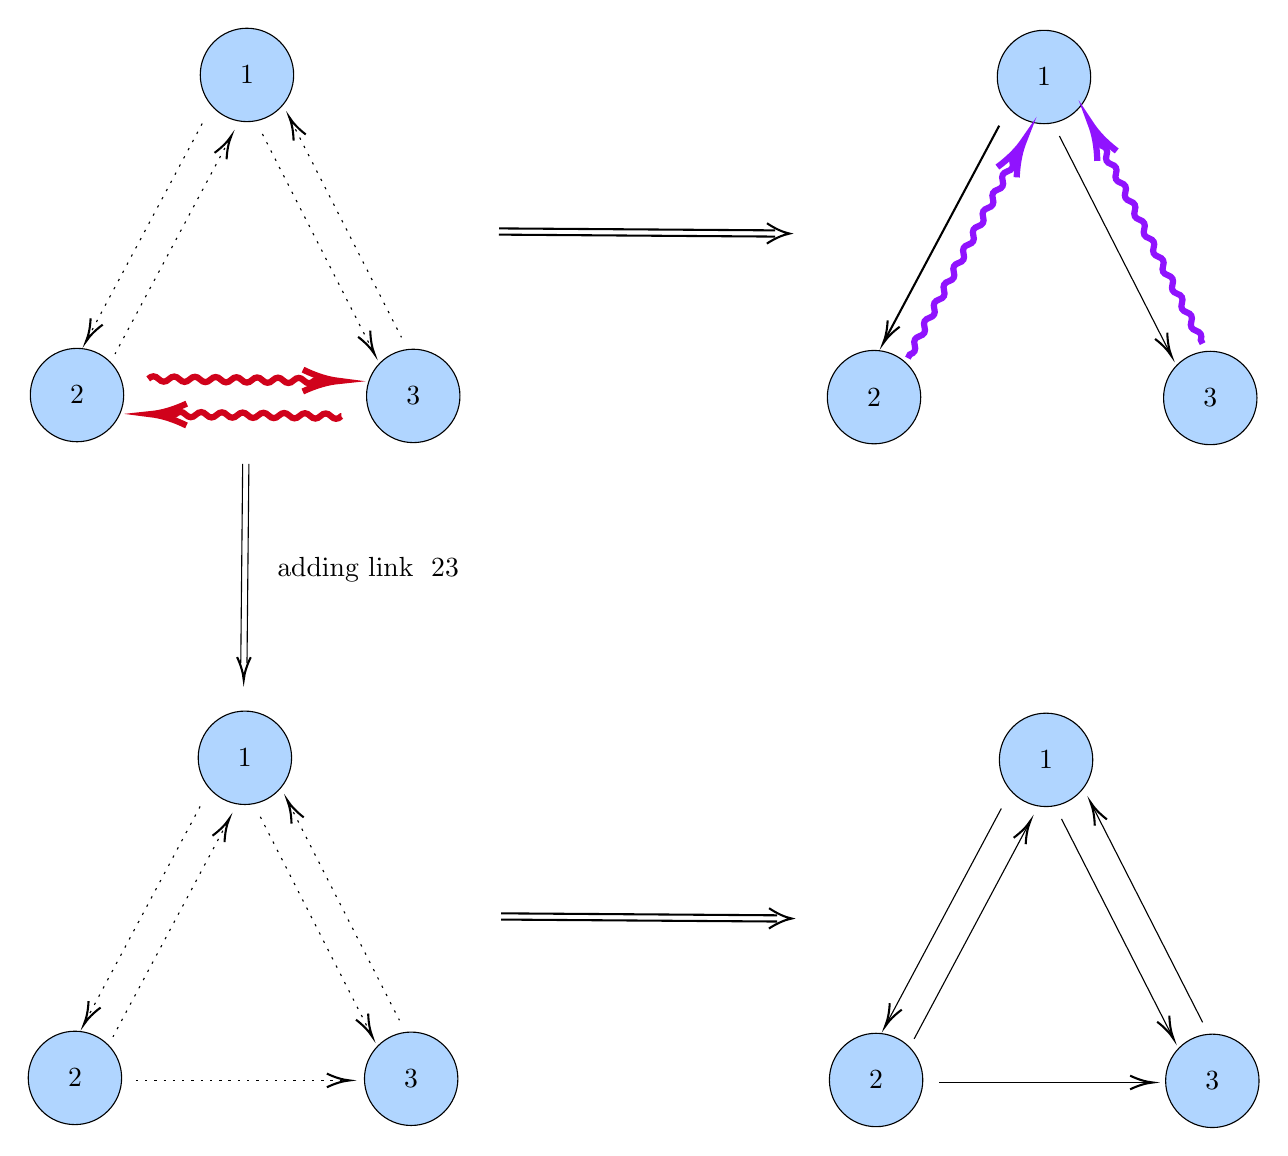
\begin{tikzpicture}[x=0.75pt,y=0.75pt,yscale=-1,xscale=1]
\draw  [fill={rgb, 255:red, 103; green, 174; blue, 255 }  ,fill opacity=0.52 ] (190.07,54.56) .. controls (190.07,42.13) and (200.15,32.06) .. (212.57,32.06) .. controls (225,32.06) and (235.07,42.13) .. (235.07,54.56) .. controls (235.07,66.98) and (225,77.06) .. (212.57,77.06) .. controls (200.15,77.06) and (190.07,66.98) .. (190.07,54.56) -- cycle ;
\draw  [fill={rgb, 255:red, 103; green, 174; blue, 255 }  ,fill opacity=0.52 ] (108.18,208.79) .. controls (108.18,196.36) and (118.25,186.29) .. (130.68,186.29) .. controls (143.1,186.29) and (153.18,196.36) .. (153.18,208.79) .. controls (153.18,221.21) and (143.1,231.29) .. (130.68,231.29) .. controls (118.25,231.29) and (108.18,221.21) .. (108.18,208.79) -- cycle ;
\draw  [fill={rgb, 255:red, 103; green, 174; blue, 255 }  ,fill opacity=0.52 ] (270.18,209.21) .. controls (270.18,196.79) and (280.25,186.71) .. (292.68,186.71) .. controls (305.1,186.71) and (315.18,196.79) .. (315.18,209.21) .. controls (315.18,221.64) and (305.1,231.71) .. (292.68,231.71) .. controls (280.25,231.71) and (270.18,221.64) .. (270.18,209.21) -- cycle ;
\draw  [dash pattern={on 0.84pt off 2.51pt}]  (191,78) -- (135.94,181.24) ;
\draw [shift={(135,183)}, rotate = 298.07] [color={rgb, 255:red, 0; green, 0; blue, 0 }  ][line width=0.75]    (10.93,-3.29) .. controls (6.95,-1.4) and (3.31,-0.3) .. (0,0) .. controls (3.31,0.3) and (6.95,1.4) .. (10.93,3.29)   ;
\draw  [dash pattern={on 0.84pt off 2.51pt}]  (204.06,85.76) -- (149,189) ;
\draw [shift={(205,84)}, rotate = 118.07] [color={rgb, 255:red, 0; green, 0; blue, 0 }  ][line width=0.75]    (10.93,-3.29) .. controls (6.95,-1.4) and (3.31,-0.3) .. (0,0) .. controls (3.31,0.3) and (6.95,1.4) .. (10.93,3.29)   ;
\draw  [dash pattern={on 0.84pt off 2.51pt}]  (220,83) -- (273.09,187.22) ;
\draw [shift={(274,189)}, rotate = 243] [color={rgb, 255:red, 0; green, 0; blue, 0 }  ][line width=0.75]    (10.93,-3.29) .. controls (6.95,-1.4) and (3.31,-0.3) .. (0,0) .. controls (3.31,0.3) and (6.95,1.4) .. (10.93,3.29)   ;
\draw  [dash pattern={on 0.84pt off 2.51pt}]  (233.91,76.78) -- (287,181) ;
\draw [shift={(233,75)}, rotate = 63] [color={rgb, 255:red, 0; green, 0; blue, 0 }  ][line width=0.75]    (10.93,-3.29) .. controls (6.95,-1.4) and (3.31,-0.3) .. (0,0) .. controls (3.31,0.3) and (6.95,1.4) .. (10.93,3.29)   ;
\draw  [fill={rgb, 255:red, 103; green, 174; blue, 255 }  ,fill opacity=0.52 ] (189.07,383.56) .. controls (189.07,371.13) and (199.15,361.06) .. (211.57,361.06) .. controls (224,361.06) and (234.07,371.13) .. (234.07,383.56) .. controls (234.07,395.98) and (224,406.06) .. (211.57,406.06) .. controls (199.15,406.06) and (189.07,395.98) .. (189.07,383.56) -- cycle ;
\draw  [fill={rgb, 255:red, 103; green, 174; blue, 255 }  ,fill opacity=0.52 ] (107.18,537.79) .. controls (107.18,525.36) and (117.25,515.29) .. (129.68,515.29) .. controls (142.1,515.29) and (152.18,525.36) .. (152.18,537.79) .. controls (152.18,550.21) and (142.1,560.29) .. (129.68,560.29) .. controls (117.25,560.29) and (107.18,550.21) .. (107.18,537.79) -- cycle ;
\draw  [fill={rgb, 255:red, 103; green, 174; blue, 255 }  ,fill opacity=0.52 ] (269.18,538.21) .. controls (269.18,525.79) and (279.25,515.71) .. (291.68,515.71) .. controls (304.1,515.71) and (314.18,525.79) .. (314.18,538.21) .. controls (314.18,550.64) and (304.1,560.71) .. (291.68,560.71) .. controls (279.25,560.71) and (269.18,550.64) .. (269.18,538.21) -- cycle ;
\draw  [dash pattern={on 0.84pt off 2.51pt}]  (190,407) -- (134.94,510.24) ;
\draw [shift={(134,512)}, rotate = 298.07] [color={rgb, 255:red, 0; green, 0; blue, 0 }  ][line width=0.75]    (10.93,-3.29) .. controls (6.95,-1.4) and (3.31,-0.3) .. (0,0) .. controls (3.31,0.3) and (6.95,1.4) .. (10.93,3.29)   ;
\draw  [dash pattern={on 0.84pt off 2.51pt}]  (203.06,414.76) -- (148,518) ;
\draw [shift={(204,413)}, rotate = 118.07] [color={rgb, 255:red, 0; green, 0; blue, 0 }  ][line width=0.75]    (10.93,-3.29) .. controls (6.95,-1.4) and (3.31,-0.3) .. (0,0) .. controls (3.31,0.3) and (6.95,1.4) .. (10.93,3.29)   ;
\draw  [dash pattern={on 0.84pt off 2.51pt}]  (219,412) -- (272.09,516.22) ;
\draw [shift={(273,518)}, rotate = 243] [color={rgb, 255:red, 0; green, 0; blue, 0 }  ][line width=0.75]    (10.93,-3.29) .. controls (6.95,-1.4) and (3.31,-0.3) .. (0,0) .. controls (3.31,0.3) and (6.95,1.4) .. (10.93,3.29)   ;
\draw  [dash pattern={on 0.84pt off 2.51pt}]  (232.91,405.78) -- (286,510) ;
\draw [shift={(232,404)}, rotate = 63] [color={rgb, 255:red, 0; green, 0; blue, 0 }  ][line width=0.75]    (10.93,-3.29) .. controls (6.95,-1.4) and (3.31,-0.3) .. (0,0) .. controls (3.31,0.3) and (6.95,1.4) .. (10.93,3.29)   ;
\draw  [fill={rgb, 255:red, 103; green, 174; blue, 255 }  ,fill opacity=0.52 ] (574.07,55.56) .. controls (574.07,43.13) and (584.15,33.06) .. (596.57,33.06) .. controls (609,33.06) and (619.07,43.13) .. (619.07,55.56) .. controls (619.07,67.98) and (609,78.06) .. (596.57,78.06) .. controls (584.15,78.06) and (574.07,67.98) .. (574.07,55.56) -- cycle ;
\draw  [fill={rgb, 255:red, 103; green, 174; blue, 255 }  ,fill opacity=0.52 ] (492.18,209.79) .. controls (492.18,197.36) and (502.25,187.29) .. (514.68,187.29) .. controls (527.1,187.29) and (537.18,197.36) .. (537.18,209.79) .. controls (537.18,222.21) and (527.1,232.29) .. (514.68,232.29) .. controls (502.25,232.29) and (492.18,222.21) .. (492.18,209.79) -- cycle ;
\draw  [fill={rgb, 255:red, 103; green, 174; blue, 255 }  ,fill opacity=0.52 ] (654.18,210.21) .. controls (654.18,197.79) and (664.25,187.71) .. (676.68,187.71) .. controls (689.1,187.71) and (699.18,197.79) .. (699.18,210.21) .. controls (699.18,222.64) and (689.1,232.71) .. (676.68,232.71) .. controls (664.25,232.71) and (654.18,222.64) .. (654.18,210.21) -- cycle ;
\draw [color={rgb, 255:red, 0; green, 0; blue, 0 }  ,draw opacity=1 ][line width=0.75]    (575,79) -- (519.94,182.24) ;
\draw [shift={(519,184)}, rotate = 298.07] [color={rgb, 255:red, 0; green, 0; blue, 0 }  ,draw opacity=1 ][line width=0.75]    (10.93,-3.29) .. controls (6.95,-1.4) and (3.31,-0.3) .. (0,0) .. controls (3.31,0.3) and (6.95,1.4) .. (10.93,3.29)   ;
\draw    (604,84) -- (657.09,188.22) ;
\draw [shift={(658,190)}, rotate = 243] [color={rgb, 255:red, 0; green, 0; blue, 0 }  ][line width=0.75]    (10.93,-3.29) .. controls (6.95,-1.4) and (3.31,-0.3) .. (0,0) .. controls (3.31,0.3) and (6.95,1.4) .. (10.93,3.29)   ;
\draw [line width=0.75]    (334.01,128.5) -- (467.01,129.45)(333.99,131.5) -- (466.99,132.45) ;
\draw [shift={(474,131)}, rotate = 180.41] [color={rgb, 255:red, 0; green, 0; blue, 0 }  ][line width=0.75]    (10.93,-4.9) .. controls (6.95,-2.3) and (3.31,-0.67) .. (0,0) .. controls (3.31,0.67) and (6.95,2.3) .. (10.93,4.9)   ;
\draw [line width=0.75]    (335.01,458.5) -- (468.01,459.45)(334.99,461.5) -- (467.99,462.45) ;
\draw [shift={(475,461)}, rotate = 180.41] [color={rgb, 255:red, 0; green, 0; blue, 0 }  ][line width=0.75]    (10.93,-4.9) .. controls (6.95,-2.3) and (3.31,-0.67) .. (0,0) .. controls (3.31,0.67) and (6.95,2.3) .. (10.93,4.9)   ;
\draw    (213.5,242.01) -- (212.58,338.01)(210.5,241.99) -- (209.58,337.99) ;
\draw [shift={(211,346)}, rotate = 270.55] [color={rgb, 255:red, 0; green, 0; blue, 0 }  ][line width=0.75]    (10.93,-3.29) .. controls (6.95,-1.4) and (3.31,-0.3) .. (0,0) .. controls (3.31,0.3) and (6.95,1.4) .. (10.93,3.29)   ;
\draw  [dash pattern={on 0.84pt off 2.51pt}]  (159,539) -- (260,539) ;
\draw [shift={(262,539)}, rotate = 180] [color={rgb, 255:red, 0; green, 0; blue, 0 }  ][line width=0.75]    (10.93,-3.29) .. controls (6.95,-1.4) and (3.31,-0.3) .. (0,0) .. controls (3.31,0.3) and (6.95,1.4) .. (10.93,3.29)   ;
\draw  [fill={rgb, 255:red, 103; green, 174; blue, 255 }  ,fill opacity=0.52 ] (575.07,384.56) .. controls (575.07,372.13) and (585.15,362.06) .. (597.57,362.06) .. controls (610,362.06) and (620.07,372.13) .. (620.07,384.56) .. controls (620.07,396.98) and (610,407.06) .. (597.57,407.06) .. controls (585.15,407.06) and (575.07,396.98) .. (575.07,384.56) -- cycle ;
\draw  [fill={rgb, 255:red, 103; green, 174; blue, 255 }  ,fill opacity=0.52 ] (493.18,538.79) .. controls (493.18,526.36) and (503.25,516.29) .. (515.68,516.29) .. controls (528.1,516.29) and (538.18,526.36) .. (538.18,538.79) .. controls (538.18,551.21) and (528.1,561.29) .. (515.68,561.29) .. controls (503.25,561.29) and (493.18,551.21) .. (493.18,538.79) -- cycle ;
\draw  [fill={rgb, 255:red, 103; green, 174; blue, 255 }  ,fill opacity=0.52 ] (655.18,539.21) .. controls (655.18,526.79) and (665.25,516.71) .. (677.68,516.71) .. controls (690.1,516.71) and (700.18,526.79) .. (700.18,539.21) .. controls (700.18,551.64) and (690.1,561.71) .. (677.68,561.71) .. controls (665.25,561.71) and (655.18,551.64) .. (655.18,539.21) -- cycle ;
\draw    (576,408) -- (520.94,511.24) ;
\draw [shift={(520,513)}, rotate = 298.07] [color={rgb, 255:red, 0; green, 0; blue, 0 }  ][line width=0.75]    (10.93,-3.29) .. controls (6.95,-1.4) and (3.31,-0.3) .. (0,0) .. controls (3.31,0.3) and (6.95,1.4) .. (10.93,3.29)   ;
\draw    (589.06,415.76) -- (534,519) ;
\draw [shift={(590,414)}, rotate = 118.07] [color={rgb, 255:red, 0; green, 0; blue, 0 }  ][line width=0.75]    (10.93,-3.29) .. controls (6.95,-1.4) and (3.31,-0.3) .. (0,0) .. controls (3.31,0.3) and (6.95,1.4) .. (10.93,3.29)   ;
\draw    (605,413) -- (658.09,517.22) ;
\draw [shift={(659,519)}, rotate = 243] [color={rgb, 255:red, 0; green, 0; blue, 0 }  ][line width=0.75]    (10.93,-3.29) .. controls (6.95,-1.4) and (3.31,-0.3) .. (0,0) .. controls (3.31,0.3) and (6.95,1.4) .. (10.93,3.29)   ;
\draw    (619.91,406.78) -- (673,511) ;
\draw [shift={(619,405)}, rotate = 63] [color={rgb, 255:red, 0; green, 0; blue, 0 }  ][line width=0.75]    (10.93,-3.29) .. controls (6.95,-1.4) and (3.31,-0.3) .. (0,0) .. controls (3.31,0.3) and (6.95,1.4) .. (10.93,3.29)   ;
\draw    (546,540) -- (647,540) ;
\draw [shift={(649,540)}, rotate = 180] [color={rgb, 255:red, 0; green, 0; blue, 0 }  ][line width=0.75]    (10.93,-3.29) .. controls (6.95,-1.4) and (3.31,-0.3) .. (0,0) .. controls (3.31,0.3) and (6.95,1.4) .. (10.93,3.29)   ;
\draw [color={rgb, 255:red, 208; green, 2; blue, 27 }  ,draw opacity=1 ][line width=2.25]    (165,201) .. controls (166.68,199.35) and (168.35,199.37) .. (170,201.05) .. controls (171.65,202.74) and (173.31,202.76) .. (175,201.11) .. controls (176.68,199.46) and (178.35,199.48) .. (180,201.16) .. controls (181.65,202.85) and (183.31,202.87) .. (185,201.22) .. controls (186.68,199.57) and (188.35,199.59) .. (190,201.27) .. controls (191.65,202.96) and (193.31,202.98) .. (195,201.33) .. controls (196.68,199.68) and (198.35,199.7) .. (200,201.38) .. controls (201.65,203.06) and (203.32,203.08) .. (205,201.43) .. controls (206.69,199.78) and (208.35,199.8) .. (210,201.49) .. controls (211.65,203.17) and (213.32,203.19) .. (215,201.54) .. controls (216.69,199.89) and (218.35,199.91) .. (220,201.6) .. controls (221.65,203.28) and (223.32,203.3) .. (225,201.65) .. controls (226.69,200) and (228.35,200.02) .. (230,201.71) .. controls (231.65,203.39) and (233.32,203.41) .. (235,201.76) .. controls (236.69,200.11) and (238.35,200.13) .. (240,201.82) .. controls (241.65,203.5) and (243.32,203.52) .. (245,201.87) -- (245,201.87) -- (253,201.96) ;
\draw [shift={(257,202)}, rotate = 180.62] [color={rgb, 255:red, 208; green, 2; blue, 27 }  ,draw opacity=1 ][line width=2.25]    (17.49,-5.26) .. controls (11.12,-2.23) and (5.29,-0.48) .. (0,0) .. controls (5.29,0.48) and (11.12,2.23) .. (17.49,5.26)   ;
\draw [color={rgb, 255:red, 208; green, 2; blue, 27 }  ,draw opacity=1 ][line width=2.25]    (170,218.04) -- (178,218.13) .. controls (179.68,216.48) and (181.35,216.5) .. (183,218.18) .. controls (184.65,219.87) and (186.31,219.89) .. (188,218.24) .. controls (189.68,216.59) and (191.35,216.61) .. (193,218.29) .. controls (194.65,219.98) and (196.31,220) .. (198,218.35) .. controls (199.68,216.7) and (201.35,216.72) .. (203,218.4) .. controls (204.65,220.09) and (206.31,220.11) .. (208,218.46) .. controls (209.68,216.81) and (211.35,216.83) .. (213,218.51) .. controls (214.65,220.2) and (216.31,220.22) .. (218,218.57) .. controls (219.68,216.92) and (221.35,216.94) .. (223,218.62) .. controls (224.65,220.3) and (226.32,220.32) .. (228,218.67) .. controls (229.69,217.02) and (231.35,217.04) .. (233,218.73) .. controls (234.65,220.41) and (236.32,220.43) .. (238,218.78) .. controls (239.69,217.13) and (241.35,217.15) .. (243,218.84) .. controls (244.65,220.52) and (246.32,220.54) .. (248,218.89) .. controls (249.69,217.24) and (251.35,217.26) .. (252.99,218.95) .. controls (254.64,220.63) and (256.31,220.65) .. (257.99,219) -- (258,219) -- (258,219) ;
\draw [shift={(166,218)}, rotate = 0.62] [color={rgb, 255:red, 208; green, 2; blue, 27 }  ,draw opacity=1 ][line width=2.25]    (17.49,-5.26) .. controls (11.12,-2.23) and (5.29,-0.48) .. (0,0) .. controls (5.29,0.48) and (11.12,2.23) .. (17.49,5.26)   ;
\draw [color={rgb, 255:red, 144; green, 19; blue, 254 }  ,draw opacity=1 ][line width=2.25]    (585.12,89.53) -- (581.35,96.59) .. controls (582.04,98.84) and (581.25,100.31) .. (579,101) .. controls (576.75,101.69) and (575.96,103.16) .. (576.65,105.41) .. controls (577.33,107.66) and (576.54,109.13) .. (574.29,109.82) .. controls (572.04,110.51) and (571.25,111.99) .. (571.94,114.24) .. controls (572.63,116.49) and (571.84,117.96) .. (569.59,118.65) .. controls (567.34,119.34) and (566.55,120.81) .. (567.24,123.06) .. controls (567.92,125.31) and (567.13,126.78) .. (564.88,127.47) .. controls (562.63,128.16) and (561.84,129.63) .. (562.53,131.88) .. controls (563.22,134.13) and (562.43,135.6) .. (560.18,136.29) .. controls (557.92,136.98) and (557.13,138.45) .. (557.82,140.71) .. controls (558.51,142.96) and (557.72,144.43) .. (555.47,145.12) .. controls (553.22,145.81) and (552.43,147.28) .. (553.12,149.53) .. controls (553.8,151.78) and (553.01,153.25) .. (550.76,153.94) .. controls (548.51,154.63) and (547.72,156.1) .. (548.41,158.35) .. controls (549.1,160.6) and (548.31,162.07) .. (546.06,162.76) .. controls (543.81,163.45) and (543.02,164.93) .. (543.71,167.18) .. controls (544.39,169.43) and (543.6,170.9) .. (541.35,171.59) .. controls (539.1,172.28) and (538.31,173.75) .. (539,176) .. controls (539.69,178.25) and (538.9,179.72) .. (536.65,180.41) .. controls (534.4,181.1) and (533.61,182.57) .. (534.29,184.82) .. controls (534.98,187.07) and (534.19,188.55) .. (531.94,189.24) -- (531,191) -- (531,191) ;
\draw [shift={(587,86)}, rotate = 118.07] [color={rgb, 255:red, 144; green, 19; blue, 254 }  ,draw opacity=1 ][line width=2.25]    (17.49,-5.26) .. controls (11.12,-2.23) and (5.29,-0.48) .. (0,0) .. controls (5.29,0.48) and (11.12,2.23) .. (17.49,5.26)   ;
\draw [color={rgb, 255:red, 144; green, 19; blue, 254 }  ,draw opacity=1 ][line width=2.25]    (620.82,81.56) -- (624.45,88.69) .. controls (626.69,89.42) and (627.45,90.91) .. (626.72,93.15) .. controls (625.99,95.39) and (626.75,96.87) .. (628.99,97.6) .. controls (631.23,98.33) and (631.99,99.82) .. (631.26,102.06) .. controls (630.53,104.3) and (631.29,105.78) .. (633.53,106.51) .. controls (635.77,107.24) and (636.53,108.73) .. (635.8,110.97) .. controls (635.07,113.21) and (635.82,114.69) .. (638.06,115.42) .. controls (640.3,116.15) and (641.06,117.64) .. (640.33,119.88) .. controls (639.6,122.12) and (640.36,123.6) .. (642.6,124.33) .. controls (644.84,125.06) and (645.6,126.55) .. (644.87,128.79) .. controls (644.14,131.03) and (644.9,132.51) .. (647.14,133.24) .. controls (649.38,133.97) and (650.14,135.46) .. (649.41,137.7) .. controls (648.68,139.94) and (649.44,141.42) .. (651.68,142.15) .. controls (653.92,142.88) and (654.68,144.37) .. (653.95,146.61) .. controls (653.22,148.85) and (653.98,150.34) .. (656.22,151.07) .. controls (658.46,151.8) and (659.22,153.28) .. (658.49,155.52) .. controls (657.76,157.76) and (658.52,159.25) .. (660.76,159.98) .. controls (663,160.71) and (663.76,162.19) .. (663.03,164.43) .. controls (662.3,166.67) and (663.06,168.16) .. (665.3,168.89) .. controls (667.54,169.62) and (668.3,171.1) .. (667.57,173.34) .. controls (666.84,175.58) and (667.6,177.07) .. (669.84,177.8) .. controls (672.08,178.53) and (672.84,180.01) .. (672.11,182.25) -- (673,184) -- (673,184) ;
\draw [shift={(619,78)}, rotate = 63] [color={rgb, 255:red, 144; green, 19; blue, 254 }  ,draw opacity=1 ][line width=2.25]    (17.49,-5.26) .. controls (11.12,-2.23) and (5.29,-0.48) .. (0,0) .. controls (5.29,0.48) and (11.12,2.23) .. (17.49,5.26)   ;
\draw (260,293) node   [align=left] {adding link};
\draw (308,292) node    {$23$};
\draw (676.68,210.21) node    {$3$};
\draw (514.68,209.79) node    {$2$};
\draw (596.57,55.56) node    {$1$};
\draw (291.68,538.21) node    {$3$};
\draw (129.68,537.79) node    {$2$};
\draw (211.57,383.56) node    {$1$};
\draw (292.68,209.21) node    {$3$};
\draw (130.68,208.79) node    {$2$};
\draw (212.57,54.56) node    {$1$};
\draw (677.68,539.21) node    {$3$};
\draw (515.68,538.79) node    {$2$};
\draw (597.57,384.56) node    {$1$};
\end{tikzpicture}}
\caption{Key adding link in endogenous and exogenous network}
\end{figure}
\end{frame}


\section{Conclusion}

\begin{frame}{Conclusion}
\begin{itemize}
    \item We consider the endogenous network formation with peer effect
    \item In the model, link formation costs play an important role in determining the network structure and individual and aggregate behaviors
    \item Due to the supermodularity, we can show the existence of equilibrium network
    \item We can provide
    \begin{itemize}
        \item comparative statics result
        \item discussion about policy implication
    \end{itemize}
\end{itemize}
\end{frame}

\begin{frame}{Future work}
\begin{itemize}
    \item link formation with bilateral agreement
    \item weighted network
    \item other form of utility function
\end{itemize}
\end{frame}


\section{Appendix}

\begin{frame}[label=proof]{Proof of the theorem}
\begin{itemize}
    \item {\bf{Lemma 1}} : Consider the network $g$ and $\hat{g}$ with $g \subseteq \hat{g}$. Then,
            \[ \bm{x}^*(\hat{g}) \ge \bm{x}^*(g) \]
    \item {\bf{Lemma 2}} : Consider the network $g$, $\hat{g}$, $h$, and $\hat{h}$ ($\bm{G}$, $\bm{\hat{G}}$, $\bm{H}$, and $\bm{\hat{H}}$) such that $\bm{G} \ge \bm{H}$ and  $\bm{\hat{G}} \ge \bm{\hat{H}}$ with $\bm{\hat{G}} - \bm{G} = \bm{\hat{H}} - \bm{H}$. Then,
            \[ v_i^*(\bm{x}^*(\hat{g}), \hat{g}, \phi) - v_i^*(\bm{x}^*(g), g, \phi) \ge v_i^*(\bm{x}^*(\hat{h}), \hat{h}, \phi) - v_i^*(\bm{x}^*(h), h, \phi)\]
\end{itemize}
\end{frame}

\begin{frame}{Proof of Lemma 2}
\begin{itemize}
    \item Let $\bm{D} = \bm{\hat{G}} - \bm{G} = \bm{\hat{H}} - \bm{H}$
    \item Then,
        \begin{eqnarray*}
            \bm{x}^*(\hat{g}) - \bm{x}^*(g) &=& {(\bm{I} - \phi \bm{\hat{G}})}^{-1} \bm{\alpha} - {(\bm{I} - \phi \bm{G})}^{-1} \bm{\alpha} \\
                                            &=& \sum_{p=0}^{\infty} \phi^p (\bm{\hat{G}}^p - \bm{G}^p) \bm{\alpha} \\
                                            &=& \phi \bm{D} \bm{\alpha} + \phi^2 \{ \bm{GD} + \bm{DG} + \bm{D}^2 \} \bm{\alpha} + \cdots
        \end{eqnarray*}
    \item Similarly,
        \[ \bm{x}^*(\hat{h}) - \bm{x}^*(h) = \phi \bm{D} \bm{\alpha} + \phi^2 \{ \bm{HD} + \bm{DH} + \bm{D}^2 \} \bm{\alpha} + \cdots \]
    \item Therefore,
        \[ \{ \bm{x}^*(\hat{g}) - \bm{x}^*(g) \} - \{ \bm{x}^*(\hat{h}) - \bm{x}^*(h) \} = \phi^2 \{(\bm{G} - \bm{H}) \bm{D} + \bm{D} (\bm{G} - \bm{H})\} \bm{\alpha} + \cdots \]
\end{itemize}
\end{frame}

\begin{frame}{Proof of Lemma 2}
\begin{itemize}
    \item Since $\bm{G} - \bm{H}$ and $\bm{D}$ is nonnegative matrix, we have
        \[ \bm{x}^*(\hat{g}) - \bm{x}^*(g) \ge \bm{x}^*(\hat{h}) - \bm{x}^*(h) \]
    \item By Lemma 1, we have
        \[ \bm{x}^*(\hat{g}) + \bm{x}^*(g) \ge \bm{x}^*(\hat{h}) + \bm{x}^*(h) \]
    \item Therefore,
        \[ v_i^*(\bm{x}^*(\hat{g}), \hat{g}, \phi) - v_i^*(\bm{x}^*(g), g, \phi) \ge v_i^*(\bm{x}^*(\hat{h}), \hat{h}, \phi) - v_i^*(\bm{x}^*(h), h, \phi)\]
\end{itemize}
\end{frame}

\begin{frame}{Proof of the theorem}
\begin{itemize}
    \item $\Gamma = \langle N, \bm{\Psi}, {(u_i)}_{i \in N} \rangle$ $\rightarrow$ $\bm{\Psi}$ is sublattice of $\prod_{i=1}^n \mathbb{R}^n$
    \item increasing differences $\rightarrow$ Lemma 2
    \item supermodularity of $u_i(\psi_i, \psi_{-i})$ in $\psi_i$
    \begin{itemize}
        \item Take any $\psi_i, \psi_i' \in \Psi_i$
        \item Consider $g=g(\psi_i,\psi_{-i})$ and $h=g(\psi_i \wedge \psi_i',\psi_{-i})$ ($\bm{G}$ and $\bm{H}$)
        \item Consider the nonnegative matrix $\bm{D}$ with
            \[ d_{ij} = \begin{cases}
                    1 & (\text{if} \ g_{ij} = 1 \ \text{and} \ h_{ij} = 0) \\
                    0 & (\text{otherwise})
                \end{cases} \]
        \item Then,the adjacency matrix of $g(\psi_i \vee \psi_i', \psi_{-i})$ and $g(\psi_i, \psi_{-i})$ are $\bm{G} + \bm{D}$ and $\bm{H} + \bm{D}$ respectively
        \item By Lemma 2,
            {\footnotesize
            \[ v_i(g(\psi_i', \psi_{-i}), \phi) - v_i(g(\psi_i \wedge \psi_i', \psi_{-i}), \phi) \le v_i(g(\psi_i \vee \psi_i', \psi_{-i}), \phi) - v_i(g(\psi_i, \psi_{-i}), \phi) \]
            }
    \end{itemize}
    \hyperlink{theorem}{[Back]}
\end{itemize}
\end{frame}


\end{document}